%!TEX root = ../Thesis.tex

% This information is used in titlepage, colophon, preface and hyperref setup (pdf metainfo), and other options.

%\def\thesistypeabbr{B.Eng.}
%\def\thesistype    {Bachelor of Engineering}
%\def\thesistypeabbr{B.Sc.Eng.}
%\def\thesistype    {Bachelor of Science in Engineering}
\def\thesistypeabbr{M.Sc.}
\def\thesistype    {Master of Science in Engineering}
%\def\thesistypeabbr{Ph.D.}
%\def\thesistype    {Doctor of Philosophy}

\def\thesisauthor  {Eleftherios Katiforis (s222725)}
\def\thesistitle   {Logical Fallacy Detection using LLMs}
\def\thesissubtitle{Master Thesis}
\def\thesislocation{Kongens Lyngby}

\def\papersize    {b5paper} % Final papersize (b5paper/a4paper), recommended papersize for DTU Compute is b5paper
\def\showtrims    {false} % Print on larger paper than \papersize and show trim marks (true/false)?

\def\showtodos    {true}  % Show todos (true/false)?
\def\confidential {false} % Confidential thesis (true/false)?



%!TEX TS-program = xelatex
%!TEX root = ../Thesis.tex
\RequirePackage[l2tabu,orthodox]{nag} % Old habits die hard

\newcommand{\papersizeswitch}[3]{\ifnum\strcmp{\papersize}{#1}=0#2\else#3\fi}
\papersizeswitch{b5paper}{\def\classfontsize{10pt}}{\def\classfontsize{12pt}}

\documentclass[\papersize,oneside,openany,showtrims,extrafontsizes]{memoir}

% %!TEX root = ../Thesis.tex
% \RequirePackage[l2tabu,orthodox]{nag} % Old habits die hard

% \newcommand{\papersizeswitch}[3]{\ifnum\strcmp{\papersize}{#1}=0#2\else#3\fi}
% \papersizeswitch{b5paper}{\def\classfontsize{10pt}}{\def\classfontsize{12pt}}

% \documentclass[\classfontsize,\papersize,twoside,showtrims,extrafontsizes]{memoir}
\RequireXeTeX

\showtrimsoff
\papersizeswitch{b5paper}{
    % Stock and paper layout
    \pagebv
    \setlrmarginsandblock{26mm}{20mm}{*}
    \setulmarginsandblock{35mm}{30mm}{*}
    \setheadfoot{8mm}{10mm}
    \setlength{\headsep}{7mm}
    \setlength{\marginparwidth}{18mm}
    \setlength{\marginparsep}{2mm}
}{
    \papersizeswitch{a4paper}{
        \pageaiv
        \setlength{\trimtop}{0pt}
        \setlength{\trimedge}{\stockwidth}
        \addtolength{\trimedge}{-\paperwidth}
        \settypeblocksize{634pt}{448.13pt}{*}
        \setulmargins{4cm}{*}{*}
        \setlrmargins{*}{*}{0.66}
        \setmarginnotes{17pt}{51pt}{\onelineskip}
        \setheadfoot{\onelineskip}{2\onelineskip}
        \setheaderspaces{*}{2\onelineskip}{*}
    }{
    }
}
\ifnum\strcmp{\showtrims}{true}=0
    % For printing B5 on A4 with trimmarks
    \showtrimson
    \papersizeswitch{b5paper}{\stockaiv}{\stockaiii}
    \setlength{\trimtop}{\stockheight}
    \addtolength{\trimtop}{-\paperheight}
    \setlength{\trimtop}{0.5\trimtop}
    \setlength{\trimedge}{\stockwidth}
    \addtolength{\trimedge}{-\paperwidth}
    \setlength{\trimedge}{0.5\trimedge}
    
    % bigger todos if trim marks
    \setmarginnotes{10pt}{95pt}{\onelineskip}

    \trimLmarks
    
    % put jobname in left top trim mark
    \renewcommand*{\tmarktl}{%
      \begin{picture}(0,0)
        \unitlength 1mm
        \thinlines
        \put(-2,0){\line(-1,0){18}}
        \put(0,2){\line(0,1){18}}
        \put(3,15){\normalfont\ttfamily\fontsize{8bp}{10bp}\selectfont\jobname\ \
          \today\ \ 
          \printtime\ \ 
          Page \thepage}
      \end{picture}}

    % Remove middle trim marks for cleaner layout
    \renewcommand*{\tmarktm}{}
    \renewcommand*{\tmarkml}{}
    \renewcommand*{\tmarkmr}{}
    \renewcommand*{\tmarkbm}{}
\fi

\checkandfixthelayout                 % Check if errors in paper format!
\sideparmargin{outer}                 % Put sidemargins in outer position (why the fuck is this option not default by the class?)

% Large environments
\usepackage{microtype}
\usepackage{mathtools}
\usepackage{listings}                 % Source code printer for LaTeX
\usepackage{tikz}
\usepackage[english]{nomencl}


% Links
\usepackage[hyphens]{url}             % Allow hyphens in URL's
\usepackage[unicode=false,psdextra]{hyperref}                 % References package

% Graphics and colors
\usepackage{graphicx}                 % Including graphics and using colours
\usepackage{xcolor}                   % Defined more color names
\usepackage{eso-pic}                  % Watermark and other bag
\usepackage{preamble/dtucolors}
\graphicspath{{graphics/}}

% Language
\usepackage{polyglossia}    % multilingual typesetting and appropriate hyphenation
\setdefaultlanguage{english}
%\usepackage{csquotes}       % language sensitive quotation facilities

% Bibliography (references)
%\usepackage[ backend=biber, style=numeric,sorting=ynt]{biblatex}

\usepackage[backend=biber,
            style=numeric,
            %backref=true,
            abbreviate=false,
            dateabbrev=false,
            alldates=long]{biblatex}
            
\usepackage{authblk}
            
%\usepackage{biblatex}
%\usepackage[numbers]{natbib}
%\usepackage{cite} 


%\usepackage{subfig}
%\usepackage{caption}
%\usepackage{subcaption}
%\captionsetup{compatibility=false}


% Floating objets, captions and references
\usepackage{flafter}  % floats is positioned after or where it is defined! 
%\setfloatlocations{figure}{bhtp}   % Set floats for all figures
%\setfloatlocations{table}{bhtp}    % Set floats for all tables
%\setFloatBlockFor{section}         % Typeset floats before each section
\usepackage[noabbrev,nameinlink,capitalise]{cleveref} % Clever references. Options: "fig. !1!" --> "!Figure 1!"
\hangcaption
\captionnamefont{\bfseries}
\subcaptionlabelfont{\bfseries}
\newsubfloat{figure}
\newsubfloat{table}
%\letcountercounter{figure}{table}         % Consecutive table and figure numbering
%\letcountercounter{lstlisting}{table}     % Consecutive table and listings numbering
\captiontitlefinal{.}
% strip things from equation references, making them "(1)" instead of "Equation~1"
% from http://tex.stackexchange.com/questions/122174/how-to-strip-eq-from-cleveref
\crefformat{equation}{(#2#1#3)}
\crefrangeformat{equation}{(#3#1#4) to~(#5#2#6)}
\crefmultiformat{equation}{(#2#1#3)}%
{ and~(#2#1#3)}{, (#2#1#3)}{ and~(#2#1#3)}

% Table of contents (TOC)
\setcounter{tocdepth}{1}              % Depth of table of content
\setcounter{secnumdepth}{2}           % Depth of section numbering
\setcounter{maxsecnumdepth}{3}        % Max depth of section numbering

\begin{comment}

% Todos
\usepackage{totcount}                 % For total counting of counters
\def\todoshowing{}
\ifnum\strcmp{\showtodos}{false}=0
    \def\todoshowing{disable}
\fi
\usepackage[colorinlistoftodos,\todoshowing]{todonotes} % Todonotes package for nice todos
\newtotcounter{todocounter}           % Creates counter in todo
\let\oldtodo\todo
\newcommand*{\newtodo}[2][]{\stepcounter{todocounter}\oldtodo[#1]{\thesection~(\thetodocounter)~#2}}
\let\todo\newtodo
\let\oldmissingfigure\missingfigure
\newcommand*{\newmissingfigure}[2][]{\stepcounter{todocounter}\oldmissingfigure[#1]{\thesection~(\thetodocounter)~#2}}
\let\missingfigure\newmissingfigure
\makeatletter
\newcommand*{\mylistoftodos}{% Only show list if there are todos
\if@todonotes@disabled
\else
    \ifnum\totvalue{todocounter}>0
        \markboth{\@todonotes@todolistname}{\@todonotes@todolistname}
        \phantomsection\todototoc
        \listoftodos
    \else
    \fi
\fi
}
\makeatother
\newcommand{\lesstodo}[2][]{\todo[color=green!40,#1]{#2}}
\newcommand{\moretodo}[2][]{\todo[color=red!40,#1]{#2}}
\end{comment}


%%%%%%%%%%%%55------------------------- My addittions for python script ---------------------

\usepackage{listings}
\usepackage{xcolor}

\definecolor{codegreen}{rgb}{0,0.6,0}
\definecolor{codegray}{rgb}{0.5,0.5,0.5}
\definecolor{codepurple}{rgb}{0.58,0,0.82}
\definecolor{backcolour}{rgb}{0.95,0.95,0.92}

\lstdefinestyle{mystyle}{
    backgroundcolor=\color{backcolour},   
    commentstyle=\color{codegreen},
    keywordstyle=\color{magenta},
    numberstyle=\tiny\color{codegray},
    stringstyle=\color{codepurple},
    basicstyle=\ttfamily\footnotesize,
    breakatwhitespace=false,         
    breaklines=true,                 
    captionpos=b,                    
    keepspaces=true,                 
    numbers=left,                    
    numbersep=5pt,                  
    showspaces=false,                
    showstringspaces=false,
    showtabs=false,                  
    tabsize=2
}

\lstset{style=mystyle}


%%%%%%%%%------------------------------------------------------------------------------------------



% Chapterstyle
\makeatletter
\makechapterstyle{mychapterstyle}{
    \chapterstyle{default}
    \def\format{\normalfont\sffamily}

    \setlength\beforechapskip{0mm}

    \renewcommand*{\chapnamefont}{\format\HUGE}
    \renewcommand*{\chapnumfont}{\format\fontsize{54}{54}\selectfont}
    \renewcommand*{\chaptitlefont}{\format\fontsize{42}{42}\selectfont}

    \renewcommand*{\printchaptername}{\chapnamefont\MakeUppercase{\@chapapp}}
    \patchcommand{\printchaptername}{\begingroup\color{dtugray}}{\endgroup}
    \renewcommand*{\chapternamenum}{\space\space}
    \patchcommand{\printchapternum}{\begingroup\color{dtured}}{\endgroup}
    \renewcommand*{\printchapternonum}{%
        \vphantom{\printchaptername\chapternamenum\chapnumfont 1}
        \afterchapternum
    }

    \setlength\midchapskip{1ex}

    \renewcommand*{\printchaptertitle}[1]{\raggedleft \chaptitlefont ##1}
    \renewcommand*{\afterchaptertitle}{\vskip0.5\onelineskip \hrule \vskip1.3\onelineskip}
}
\makeatother
\chapterstyle{mychapterstyle}

% Header and footer
\def\hffont{\sffamily\small}
\makepagestyle{myruled}
\makeheadrule{myruled}{\textwidth}{\normalrulethickness}
\makeevenhead{myruled}{\hffont\thepage}{}{\hffont\leftmark}
\makeoddhead{myruled}{\hffont\rightmark}{}{\hffont\thepage}
\makeevenfoot{myruled}{}{}{}
\makeoddfoot{myruled}{}{}{}
\makepsmarks{myruled}{
    \nouppercaseheads
    \createmark{chapter}{both}{shownumber}{}{\space}
    \createmark{section}{right}{shownumber}{}{\space}
    \createplainmark{toc}{both}{\contentsname}
    \createplainmark{lof}{both}{\listfigurename}
    \createplainmark{lot}{both}{\listtablename}
    \createplainmark{bib}{both}{\bibname}
    \createplainmark{index}{both}{\indexname}
    \createplainmark{glossary}{both}{\glossaryname}
}
\pagestyle{myruled}
\copypagestyle{cleared}{myruled}      % When \cleardoublepage, use myruled instead of empty
\makeevenhead{cleared}{\hffont\thepage}{}{} % Remove leftmark on cleared pages

\makeevenfoot{plain}{}{}{}            % No page number on plain even pages (chapter begin)
\makeoddfoot{plain}{}{}{}             % No page number on plain odd pages (chapter begin)

% \*section, \*paragraph font styles
\setsecheadstyle              {\huge\sffamily\raggedright}
\setsubsecheadstyle           {\LARGE\sffamily\raggedright}
\setsubsubsecheadstyle        {\Large\sffamily\raggedright}
%\setparaheadstyle             {\normalsize\sffamily\itseries\raggedright}
%\setsubparaheadstyle          {\normalsize\sffamily\raggedright}


% Hypersetup
\hypersetup{
    pdfauthor={\thesisauthor{}},
    pdftitle={\thesistitle{}},
    pdfsubject={\thesissubtitle{}},
    pdfdisplaydoctitle,
    bookmarksnumbered=true,
    bookmarksopen,
    breaklinks,
    linktoc=all,
    plainpages=false,
    unicode=true,
    colorlinks=false,
    citebordercolor=dtured,           % color of links to bibliography
    filebordercolor=dtured,           % color of file links
    linkbordercolor=dtured,           % color of internal links (change box color with linkbordercolor)
    urlbordercolor=s13,               % color of external links
    hidelinks,                        % Do not show boxes or colored links.
}
% Hack to make right pdfbookmark link. The normal behavior links just below the chapter title. This hack put the link just above the chapter like any other normal use of \chapter.
% Another solution can be found in http://tex.stackexchange.com/questions/59359/certain-hyperlinks-memoirhyperref-placed-too-low
\makeatletter
\renewcommand{\@memb@bchap}{%
  \ifnobibintoc\else
    \phantomsection
    \addcontentsline{toc}{chapter}{\bibname}%
  \fi
  \chapter*{\bibname}%
  \bibmark
  \prebibhook
}
\let\oldtableofcontents\tableofcontents
\newcommand{\newtableofcontents}{
    \@ifstar{\oldtableofcontents*}{
        \phantomsection\addcontentsline{toc}{chapter}{\contentsname}\oldtableofcontents*}}
\let\tableofcontents\newtableofcontents
\makeatother

% Confidential
\newcommand{\confidentialbox}[1]{
    \put(0,0){\parbox[b][\paperheight]{\paperwidth}{
        \begin{vplace}
            \centering
            \scalebox{1.3}{
                \begin{tikzpicture}
                    \node[very thick,draw=red!#1,color=red!#1,
                          rounded corners=2pt,inner sep=8pt,rotate=-20]
                          {\sffamily \HUGE \MakeUppercase{Confidential}};
                \end{tikzpicture}
            }
        \end{vplace}
    }}
}

% Prefrontmatter
\newcommand{\prefrontmatter}{
    \pagenumbering{alph}
    \ifnum\strcmp{\confidential}{true}=0
        \AddToShipoutPictureBG{\confidentialbox{10}}   % 10% classified box in background on each page
        \AddToShipoutPictureFG*{\confidentialbox{100}} % 100% classified box in foreground on first page
    \fi
}

% DTU frieze
\newcommand{\frieze}{%
    \AddToShipoutPicture*{
        \put(0,0){
            \parbox[b][\paperheight]{\paperwidth}{%
                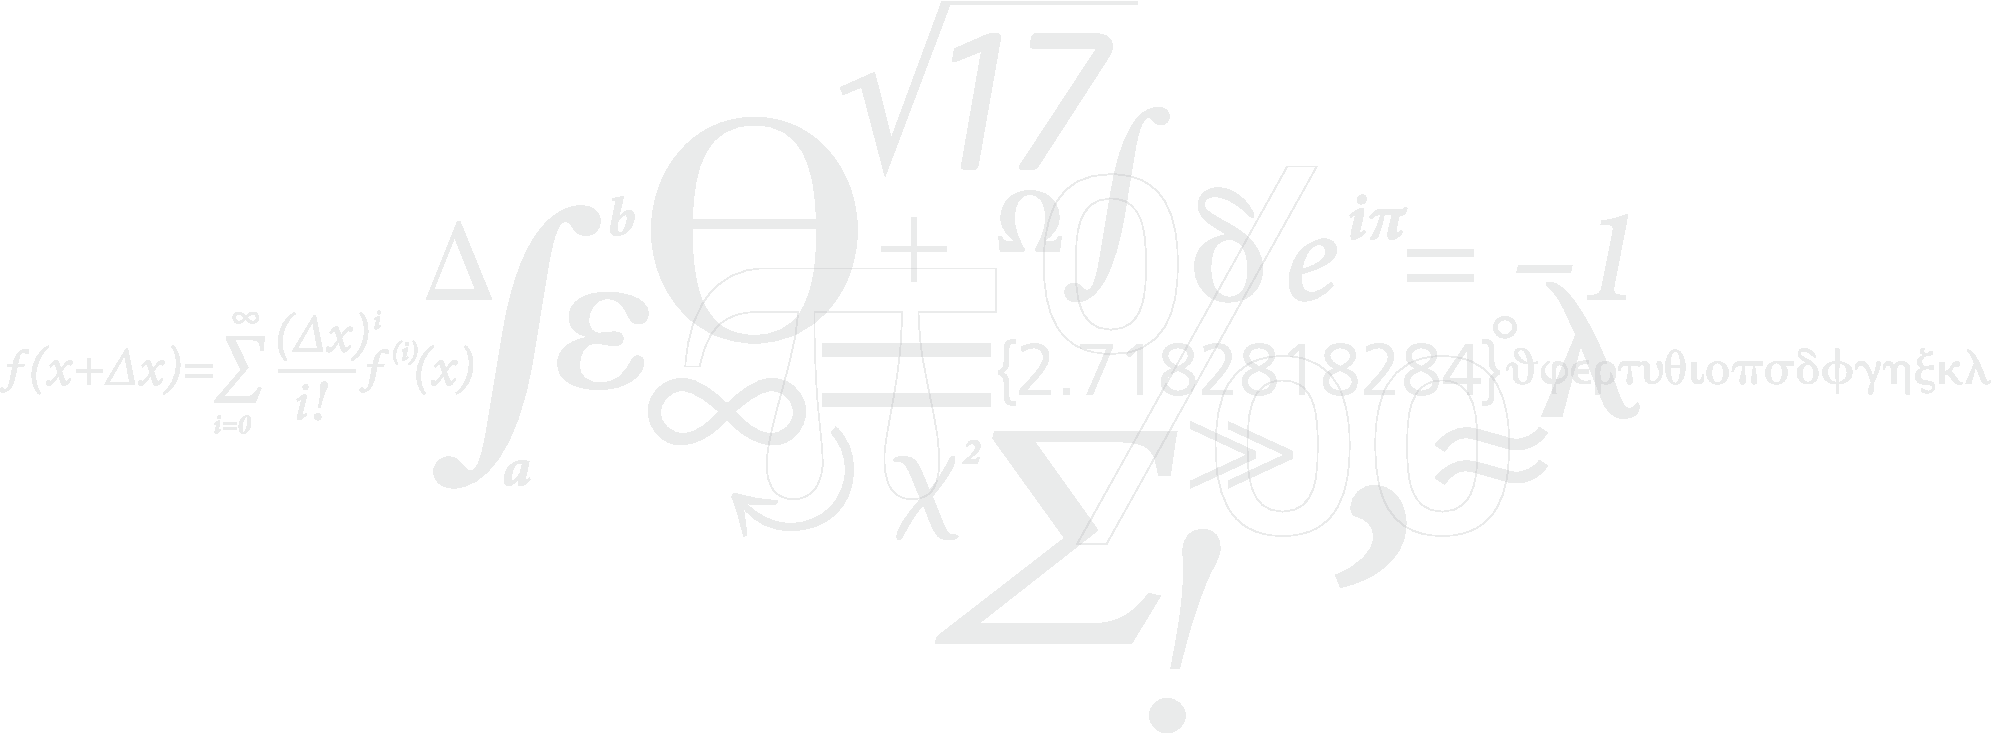
\includegraphics[trim=130mm 0 0 0,width=0.9\textwidth]{DTU-frise-SH-15}
                \vspace*{2.5cm}
            }
        }
    }
}

% This is a double sided book. If there is a last empty page lets use it for some fun e.g. the frieze.
% NB: For a fully functional hack the \clearpage used in \include does some odd thinks with the sequence numbering. Thefore use \input instead of \include at the end of the book. If bibliography is used at last everything should be ok.
\makeatletter
% Adjust so gatherings is allowd for single sheets too! (hacking functions in memoir.dtx)
\patchcmd{\leavespergathering}{\ifnum\@memcnta<\tw@}{\ifnum\@memcnta<\@ne}{
    \leavespergathering{1}
    % Insert the frieze
    \patchcmd{\@memensuresigpages}{\repeat}{\repeat\frieze}{}{}
}{}
\makeatother

%!TEX root = ../Thesis.tex

% Text fonts (http://www.macfreek.nl/memory/Fonts_in_LaTeX)
% Install fonts from /usr/local/texlive/<version>/texmf-dist/fonts/opentype/public
\usepackage{fontspec}

% Sans-serif font
\setsansfont[
    Ligatures=TeX,
    Extension=.otf,
    UprightFont=*-regular,
    BoldFont=*-bold,
    ItalicFont=*-italic,
    BoldItalicFont=*-bolditalic,
    %SlantedFont=,
    %BoldSlantedFont=,
    %SmallCapsFont=
    Scale=0.8      % Adjustmens when using math in sections
]{texgyreadventor}
%\setsansfont[Ligatures=TeX]{Neo Sans Intel}    % Neo Sans Intel – Like DTU font but more symbols
%\setsansfont[
%    Ligatures=TeX,
%    Scale=0.8
%]{NeoSans}           % NeoSans – DTU font (missing `+' symbols and other)
%\setsansfont[Ligatures=TeX]{CMU Sans Serif}    % Computer Modern Unicode font
%\setsansfont[Ligatures=TeX]{Latin Modern Sans} % Latin Modern Sans serif font

% Use this for more convienent sans serif font in math mode.
%\setmathsf{Latin Modern Sans}


%!TEX root = ../Thesis.tex

% Content specific packages.

\usepackage{blindtext}
\usepackage{algorithm}
\usepackage{algpseudocode}
\usepackage[english]{nomencl}
\usepackage{caption}
\usepackage{subcaption}
\usepackage{amssymb}
\usepackage{siunitx}
%\usepackage[acronym]{glossaries}
%\usepackage[utf8]{inputenc}


%\usepackage{pgfplots}                 % Plot tools
%\usetikzlibrary{
%    arrows,
%    matrix,
%    positioning,
%    shapes,
%    topaths,
%}
%\pgfplotsset{compat=1.7}

% Listings
\lstset{
    basicstyle=\footnotesize\ttfamily,% the size of the fonts that are used for the code
    breakatwhitespace=false,          % sets if automatic breaks should only happen at whitespace
    breaklines=true,                  % sets automatic line breaking
    captionpos=b,                     % sets the caption-position to bottom
    commentstyle=\color{s14a},        % comment style
    deletekeywords={},                % if you want to delete keywords from the given language
    escapeinside={\%*}{*)},           % if you want to add LaTeX within your code
    frame=single,                     % adds a frame around the code
    keywordstyle=\bfseries\ttfamily\color{s09}, % keyword style
    language=Python,                  % the language of the code
    morekeywords={*,...},             % if you want to add more keywords to the set
    numbers=left,                     % where to put the line-numbers; possible values are (none, left, right)
    numbersep=5pt,                    % how far the line-numbers are from the code
    numberstyle=\sffamily\tiny\color{dtugray}, % the style that is used for the line-numbers
    rulecolor=\color{dtugray},        % if not set, the frame-color may be changed on line-breaks within not-black text (e.g. comments (green here))
    showspaces=false,                 % show spaces everywhere adding particular underscores; it overrides 'showstringspaces'
    showstringspaces=false,           % underline spaces within strings only
    showtabs=false,                   % show tabs within strings adding particular underscores
    stepnumber=1,                     % the step between two line-numbers. If it's 1, each line will be numbered
    stringstyle=\color{s07},          % string literal style
    tabsize=2,                        % sets default tabsize to 2 spaces
    title=\lstname,                   % show the filename of files included with \lstinputlisting; also try caption instead of title
}



\addbibresource{bibliography/Bibliography.bib}
\renewcommand{\lstlistingname}{Python scripts}
\renewcommand{\lstlistlistingname}{List of \lstlistingname}

\begin{document}

\prefrontmatter
%!TEX root = ../Thesis.tex 
\thispagestyle{empty}             % No page numbers
\calccentering{\unitlength}
\begin{adjustwidth*}{\unitlength}{-\unitlength}
    \begin{adjustwidth}{-0.5cm}{-0.5cm}
        \sffamily
        \begin{flushright}
            \thesistypeabbr{} Thesis\\*[0cm]
            \thesistype{}\\
        \end{flushright}
        \vspace*{\fill}
        \noindent
        
\includegraphics[width=0.75\textwidth]{graphics/compute.png}\\*[0.5cm]
         \HUGE \thesistitle{}\\*[0.2cm]
        \Huge \thesissubtitle{}\\*[1.2cm]
        \parbox[b]{0.5\linewidth}{%
            \LARGE 
            \thesisauthor{}\\*[1.2cm]
            \Large
            \thesislocation{} \the\year
        }
        \hfill
\includegraphics[scale=0.7]{DTU-logo-CMYK}
    \end{adjustwidth}
\end{adjustwidth*}
\normalfont
\normalsize

\cleartoevenpage
%!TEX root = ../Thesis.tex
\thispagestyle{empty} % No page numbers
\frieze
\vspace*{\fill}
\noindent
\sffamily
\small
%\textbf{DTU Photonik}\\
%\textbf{Department of Applied Mathematics and Computer Science}\\
%\textbf{DTU Photonik}\\
%\textbf{Department of Photonics Engineering}\\
%\textbf{Technical University of Denmark}\\
\\

%Matematiktorvet\\
%Building 303B\\
%2800 Kongens Lyngby, Denmark\\
%Phone +45 4525 3031\\
%compute@compute.dtu.dk\\
%www.compute.dtu.dk\\
\noindent\textbf{Department of Applied Mathematics and Computer Science}\\
\textbf{Technical University of Denmark}\\
Richard Petersens Plads\\
Building 324, Room 160\\
2800 Kongens Lyngby, Denmark\\
%Phone Tel.: +45 45 25 52 78\\
%dimp@dtu.dk\\
www.compute.dtu.dk\\

\large
\vspace*{\fill}
\hspace{-0.52cm}\textbf{Supervisors:} %Associate Professor Dimitrios Papadopoulos\\
\vspace{5cm}

\small
% Leave the following empty spaces to avoid the Warning: "Underfull \hbox (badness 10000)"
%\hspace*{\fill}\textbf{DTU Fotonik}

%\hspace*{\fill}\textbf{Department of Photonics Engineering}

%\hspace*{\fill}\textbf{Technical University of Denmark}

%\hspace*{\fill}Ørsteds Plads

%\hspace*{\fill}Building 340

%\hspace*{\fill}2800 Kongens Lyngby, Denmark
\normalsize
\normalfont
\vspace*{2.5cm}

%\clearforchapter

\frontmatter
%!TEX root = ../Thesis.tex
\chapter{Abstract}



 
%!TEX root = ../Thesis.tex
\chapter{Preface}
%This xxx thesis was prepared at the department of Applied Mathematics and Computer Science at the Technical University of Denmark in fulfillment of the requirements for acquiring a yyy degree in zzz.

The present MSc thesis is a partial fulfillment of the requirements for the Master
of Science degree in Human-Centered Artificial Intelligence at Technical University of Denmark. \newline

\noindent The project accounts for 35 ECTS and is conducted between 4.05.2024 and 04.03.2025. The exact topic along with the objectives of the project are defined in collaboration between the author and the supervisors.

\vfill

% {
% \centering
%     \thesislocation{}, \today\\[1cm]
%     \hspace{3cm}
\includegraphics[scale=0.3]{graphics/signature.png}\\[1cm]
% \begin{flushright}
%     \thesisauthor{}
% \end{flushright}
% }
%!TEX root = ../Thesis.tex
\chapter{Acknowledgements}

%\clearforchapter
\setcounter{secnumdepth}{4}
\setcounter{tocdepth}{4}
\tableofcontents
\newpage
\listoffigures
\newpage
%\listoftables
%\newpage
%\lstlistoflistings

%\addcontentsline{toc}{chapter}{Nomenclature}
%%\chapter{Nomenclature}
\addcontentsline{toc}{chapter}{Nomenclature}
\makenomenclature
\renewcommand{\nomname}{Nomenclature}
\renewcommand{\nompreamble}{The next list describes several symbols that were used within the body of the document}
%\clearpage
%\mbox{}

%\chapter{Acronyms111111}

\nomenclature{\textbf{LoRa}}{from \textbf{Lo}ng \textbf{Ra}nge}
\nomenclature{\textbf{IoT}}{\textbf{I}nternet \textbf{o}f \textbf{T}hings}
\nomenclature{\textbf{OMNeT++}}{\textbf{O}bjective \textbf{M}odular \textbf{Ne}twork \textbf{T}estbed in C\textbf{++}}
\nomenclature{\textbf{LPWAN}}{ \textbf{L}ow-\textbf{P}ower \textbf{W}ide-\textbf{A}rea \textbf{N}etwork}
\nomenclature{\textbf{CSS}}{\textbf{C}hirp \textbf{S}pread \textbf{S}pectrum}
\nomenclature{\textbf{BW}}{\textbf{B}andwidth}
\nomenclature{\textbf{SF}}{\textbf{S}preading \textbf{F}actor}
\nomenclature{\textbf{TP}}{\textbf{T}ransmission \textbf{P}ower}
\nomenclature{\textbf{CR}}{\textbf{C}oding \textbf{R}ate}
\nomenclature{\textbf{CF}}{\textbf{C}arrier \textbf{F}requency}
\nomenclature{\textbf{SNR}}{\textbf{S}ignal to \textbf{N}oice \textbf{R}atio}
\nomenclature{\textbf{ADR}}{\textbf{A}daptive \textbf{D}ata \textbf{R}ate}
\nomenclature{\textbf{PDR}}{\textbf{P}acket \textbf{D}elivery \textbf{R}ate}
\nomenclature{\textbf{MAC}}{\textbf{M}edium \textbf{A}ccess \textbf{C}ontrol}
\nomenclature{\textbf{OTA}}{\textbf{O}ver \textbf{T}he \textbf{A}ir}
\nomenclature{\textbf{RF}}{\textbf{R}adio \textbf{F}requency}
\nomenclature{\textbf{IDE}}{\textbf{I}ntergrated \textbf{D}evelopment \textbf{E}nvironment}
\nomenclature{\textbf{GUI}}{\textbf{G}raphical \textbf{U}ser \textbf{I}nterface}
\nomenclature{\textbf{IMST}}{\textbf{I}nstitute of \textbf{M}obile and \textbf{S}atellite communication \textbf{T}echnology}
\nomenclature{\textbf{RNG}}{\textbf{R}andom \textbf{N}umber \textbf{G}enerator}
\nomenclature{\textbf{ISM}}{\textbf{I}ndustrial \textbf{S}cientific and \textbf{M}edical radio band}
\nomenclature{\textbf{GW}}{\textbf{G}ateway}

\begin{comment}

\nomenclature{VI}{Virtual Infrastracture}
\nomenclature{PI}{Physical Infrastructure}
\nomenclature{DC}{Data Center}
\nomenclature{NFV}{Network Function Virtualisation}
\nomenclature{NFVI}{Network Functions Virtualization Infrastructure}
\nomenclature{MANO}{Management, Automation and Network Orchestratio}
\nomenclature{VNF}{Virtual Network Function}
\nomenclature{SON}{Self-Organized Networks}
\nomenclature{VM}{Virtual Machine}
\nomenclature{MTTR}{Mean Time Between Failure}
\nomenclature{MTBF}{Mean Time To Repair}
\nomenclature{SLA}{Service Level Agreement}

\end{comment}

\printnomenclature
%\printnomenclature


%\clearforchapter
%\mylistoftodos

\mainmatter
%!TEX root = ../Thesis.tex
\chapter{Introduction}

Reasoning is the cognitive process of using existing knowledge to make inferences, create explanations, and assess statements rationally through logic \cite{InternetClassicsArchive}. It is fundamental to critical thinking, argumentation, and decision-making in various domains, from philosophy and science to public discourse and artificial intelligence (AI). However, human reasoning is prone to systematic errors, leading to logical fallacies—arguments that appear persuasive but are logically unsound.

Logical fallacies are prevalent in everyday life, appearing in casual conversations, advertisements, political debates, and social media. Some are harmless, such as, (source of the examples: Jin et al. \cite{jinLogicalFallacyDetection2022}):

\begin{itemize}
    \item \textbf{Faulty Generalization:} ``All tall people like cheese."
    \item \textbf{Circular Reasoning:} ``She is the best because she is better than anyone else."
\end{itemize}

However, fallacies are also intentionally exploited to manipulate opinions and spread misinformation, as seen in:

\begin{itemize}
    \item \textbf{Faulty Generalization:} ``Today is so cold, so I don’t believe in global warming."
    \item \textbf{Circular Reasoning:} ``Global warming doesn’t exist because the Earth is not getting warmer."
\end{itemize}

In an era of digital misinformation, detecting and mitigating logical fallacies is essential for rational discourse and evidence-based decision-making. Fallacy detection, once studied in philosophy and rhetoric, has now become a key challenge in computational linguistics, AI, and misinformation analysis.

Here I'll continue with the limitations and my work.




\noindent 

% 
% \chapter{Background}


\chapter{Background \& \\Related Work}

\section{Fallacy Detection}
Da San Martino et al. (2019) \cite{dasanmartinoFineGrainedAnalysisPropaganda2019} were the first to aim to detect propaganda in news articles at a granular level by identifying specific techniques used within the text, rather than labeling entire articles as propagandistic. The authors introduced a new dataset of news articles, annotated with 18 distinct propaganda techniques, such as loaded language, name calling, appeal to fear, and whataboutism. This approach enables a more detailed and explainable analysis of how propaganda operates within specific text fragments.
% Their main contributions include the creation of a corpus of news articles annotated at the fragment level with 18 propaganda techniques by expert annotators while proposing two new tasks
%  (i) Sentence-level classification (SLC), which predicts if a sentence contains propaganda, and (ii) Fragment-level classification (FLC), which identifies specific text spans and their associated propaganda techniques. Finally, they introduce a model designed to improve the detection of propaganda, outperforming several strong BERT-based baselines. This fine-grained analysis offers a more precise and explainable approach to understanding propaganda in news articles, moving beyond binary classifications of entire documents.

 Jin et al. (2022) \cite{jinLogicalFallacyDetection2022} focused on detecting logical fallacies in text, a task essential for identifying flawed reasoning that can propagate misinformation The authors introduced the LOGIC dataset, which contains 2,449 samples annotated with 13 types of logical fallacies, along with a specialized climate change dataset (LOGICCLIMATE) for fallacies found in climate discussions. Furthermore, they presented a structure-aware model that outperformed standard language models like BERT and RoBERTa in detecting logical fallacies, significantly improving the F1 score. The model focuses on the logical structure of arguments rather than just the content. 
This work focuses more on the classification of annotated samples that consist of 2-3 sentences rather than the detection of logical fallacies in large corpora of text.

 Alhindi et al. (2022) \cite{alhindiMultitaskInstructionbasedPrompting2022} explored the detection of fallacies across different types of datasets using a unified multitask framework. The main innovation of the paper was the use of instruction-based prompting with a T5 model, which enabled the model to handle 28 unique fallacies across various genres and domains by transforming them into natural language instructions. This approach significantly outperformed traditional methods trained on specific datasets or tasks, offering a broad, adaptable, and effective system for fallacy recognition.
The authors address several challenges in fallacy detection, such as dataset heterogeneity and the high number of classification labels, by unifying multiple datasets under a single framework. They demonstrate that their method not only improves the macro F1 scores by considerable margins but also provides insights into the effects of model size and prompt choices on classification accuracy. 

Vorakitphan et al. (2023) \cite{vorakitphanPROTECTPipelinePropaganda2022}  introduced PROTECT (PROpaganda Text dEteCTion), a system designed to automatically detect and classify propaganda in texts. PROTECT uses semantic and argumentation features to analyze texts for propaganda content, identifying the techniques employed.
PROTECT first identifies propaganda snippets within a given text and then classifies them based on the type of propaganda technique used. The system utilizes a transformer architecture, likely leveraging models like BERT, to perform its classification tasks.
It is evaluated using standard datasets known for propaganda analysis introduced by Da San Martino et al. (2019)\cite{dasanmartinoFineGrainedAnalysisPropaganda2019}, showing promising results.
PROTECT is equipped with a user-friendly web interface and API, making it accessible for public use and allowing for the analysis of user-submitted texts.
This work contributed to the field by providing a tool that not only automates the detection of propaganda but also helps educate the public about the nuances of manipulative content in media.

Goffredo et al. (2023) \cite{goffredoArgumentbasedDetectionClassification2023} delved into the detection and categorization of logical fallacies in political debates. The authors extended a pre-existing dataset of U.S. presidential debates to include the 2020 Trump-Biden debates, enriching it with detailed annotations of argumentative structures and fallacies.
The methodology focused on a transformer-based neural network model integrating text analysis with argumentative and engineered features, significantly improving the detection and classification of fallacies. 
The study presents a nuanced approach to handling fallacious arguments by incorporating the relations and components of the arguments, which is a novel contribution to the field of computational linguistics and argument mining.
% This advancement supports a more informed public discourse by potentially limiting the spread of manipulative or misleading political claims.

\section{Large Language Models}

\begin{enumerate}
    \item Write about LLMs, attention?
    \item Reasoning in LLMs
    \item LLMs and fallacy classification
\end{enumerate}


\section{Chain of Thought}

Wei et al. (2022) \cite{ChainThoughtPromptingElicits} introduced the concept of "Chain-of-Thought Prompting" in their paper Chain-of-Thought Prompting Elicits Reasoning in Large Language Models. This technique involves providing models with a series of intermediate reasoning steps as exemplars during In-Context Learning. Their findings showed that models with over 100 billion parameters experienced significant improvements in solving complex multi-step problems, such as arithmetic and commonsense reasoning. However, smaller models (under 100 billion parameters) not only failed to benefit from this approach but sometimes performed worse, generating fluent but illogical reasoning chains. Additionally, they observed variability in performance—sometimes as much as 20\%—due to differences in hand-crafted exemplars created by various annotators.

Building on Wei et al.'s work, Kojima et al. (2022) \cite{kojimaLargeLanguageModels2023} addressed the primary limitation of Chain-of-Thought Prompting: the dependence on hand-crafted exemplars and their associated performance variability. Their approach introduced a simple phrase, "Let’s think step-by-step," to the prompt, encouraging the model to generate logical intermediate reasoning steps. By appending these steps to the original prompt, they achieved notable performance improvements across tasks previously evaluated using Chain-of-Thought Prompting, such as arithmetic and commonsense reasoning. However, while their method reduced reliance on hand-crafted examples, it did not yield as significant a performance boost as the original approach and remained ineffective for smaller models with fewer than 100 billion parameters.
\chapter{Method}

In this chapter we describe the methodology used to evaluate the performance of the models in the task of logical fallacy detection. We begin by describing the dataset used for the experiments, followed by the models and the evaluation metrics used. We then describe the experimental setup, including the zero-shot, the categorization of the fallacies inluded in our dataset of choice, the chain-of-thought prompting and the multi-round chain of thought approach used to evaluate the models' performance.

\section{Dataset}

Missing, describe LOGIC dataset, why it was chosen and include figures.


\section{Models}

For our experiments, we selected Falcon-Mamba-7B-Instruct, Meta-Llama-3.1-8B-Instruct, and Mistral-7B-Instruct-v0.3 as our primary models. Since our work involves extremely long prompts—including fallacy names, definitions, and multi-round prompting—we needed models with strong long-context retention and instruction-following capabilities. These models were chosen for their ability to process and reason over extended input sequences while maintaining efficiency and logical coherence.
\par
Each of these models brings unique architectural strengths: Falcon-Mamba-7B-Instruct is optimized for memory-efficient state-space modeling, Meta-Llama-3.1-8B-Instruct leverages advanced positional embeddings to enhance long-sequence comprehension, and Mistral-7B-Instruct utilizes optimized attention mechanisms to improve logical reasoning across long text passages. Their instruction-tuning capabilities and proficiency in zero-shot/few-shot reasoning make them particularly well-suited for fallacy detection tasks, where nuanced reasoning over extended textual input is required.
\par
Falcon-Mamba-7B-Instruct represents a breakthrough in non-Transformer architectures, employing state-space modeling (SSM) instead of self-attention to enable scalable, memory-efficient long-context processing (Zuo et al., 2024) \cite{zuo2024falconmambacompetitiveattentionfree}. Unlike traditional LLMs, which face quadratic complexity in attention computation, Falcon-Mamba-7B uses a structured recurrence mechanism to maintain constant memory usage regardless of sequence length. This makes it highly effective for document-level reasoning and real-time applications. Additionally, it has been trained on a massive 5.8 trillion token dataset, incorporating instruction tuning, multilingual data, and domain-specific corpora, further enhancing its accuracy in complex tasks.
\par
Meta-Llama-3.1-8B-Instruct, part of the LLaMA (Large Language Model Meta AI) family, extends Transformer-based architectures by integrating Grouped Query Attention (GQA) and Rotary Positional Embeddings (RoPE), leading to improved efficiency in reasoning and long-context comprehension (Meta AI, 2024) \cite{grattafiori2024llama3herdmodels} . Trained on 15 trillion tokens, this model is fine-tuned for multilingual applications, logical inference, and structured decision-making tasks. Empirical benchmarks show that Meta-Llama-3.1-8B-Instruct outperforms earlier LLaMA models in several tasks including math reasoning andmultilingual benchmarks.
\par
Mistral-7B-Instruct-v0.3 is a highly optimized Transformer model designed to balance reasoning accuracy with inference efficiency, making it a strong alternative to larger LLMs (Jiang et al., 2023) \cite{jiang2023mistral7b}. It incorporates Sliding Window Attention (SWA) and Grouped Query Attention (GQA) to preserve context over long sequences while maintaining fast inference speeds, which is particularly beneficial for multi-step logical reasoning. Despite its relatively compact 7-billion-parameter size, Mistral-7B-Instruct delivers competitive results in code generation, commonsense reasoning, and structured question-answering, outperforming larger models while using significantly fewer computational resources.
\par
The selection of Falcon-Mamba-7B-Instruct, Meta-Llama-3.1-8B-Instruct, and Mistral-7B-Instruct-v0.3 was driven by their superior long-context reasoning capabilities, efficient processing mechanisms, and strong instruction-following performance. Each model brings distinct architectural strengths that contribute to handling the complexity of logical fallacy detection, particularly when working with extended prompts and multi-step reasoning tasks.



\section{Zero-Shot}
At first, we conducted a set of zero-shot experiments with the above-stated models. Zero-shot experiments test the capacity of a model to carry out a task without having been specifically trained on that task, thus proving to be an effective method for assessing whether these models are capabl of performing this task without any fine-tuning. To test their performance and consistency, based on previous studies suggesting that the wording of a prompt can signifcalty affect the model's response, we designed and executed two different prompts for each of the models asking forthe same task but with some minor differences in wording and on the specific instructions. The prompts, as may be accessed, were specifically designed to test the models' capacity for classifying fallacious arguments regardless of explicit supervision or exposure to labeled training data.

Furthermore, to examine the possible effect of explicit definitional instruction on the performance of the models, we included two more variations for each prompt. One variation included full definitions of the logical fallacies, with explicit explanations and contextual information about the nature and structure of each fallacy. In contrast, the second variation explicitly excluded these definitions, leaving the models to depend on their prior knowledge on te topic and reasoning capabilities alone to detect instances of fallacious argumentation.

\begin{table}[H]
    \centering
    \renewcommand{\arraystretch}{1.1}
    \captionsetup{justification=centering}
    \caption{Comparison of Zero-Shot Fallacy Detection Prompts}
    \scriptsize % Reduce text size
    \begin{tabular}{|m{0.48\textwidth}|m{0.48\textwidth}|}
        \hline
        \textbf{Prompt 1} & \textbf{Prompt 2} \\
        \hline
        \parbox[t]{0.45\textwidth}{%
            You will be provided with a text segment, delimited by \#\#\#\# characters, and your task is to classify it into one of the fallacy types listed below. \\
            
            Provide your output in JSON format with the key: `detected\_fallacy`. The value should be the name of the detected fallacy, chosen from the list below. Do not include any explanation or commentary. \\

            The \#\#\#\# characters are only delimiters for the segment. Do not include them in your classification or output. \\

            The possible fallacy types are: \\
            1. Appeal To Emotion: attempting to arouse non-rational sentiments within the intended audience in order to persuade. \\
            2. False Causality: occurs when someone mistakenly assumes that because one event follows another, the first event caused the second, without sufficient evidence for a causal link. \\
            3. Ad Hominem: The opponent attacks a person instead of arguing against the claims that the person has put forward. \\
            4. Faulty Generalization: A generalization is drawn from a sample which is too small, it is not representative of the population or it is not applicable to the situation if all the variables are taken into account. \\
            5. False Dilemma: Presenting two alternative options as the only possibilities, when in fact more possibilities exist. As an the extreme case, tell the audience exactly what actions to take, eliminating any other possible choices (Dictatorship). \\
            6. Fallacy of Relevance: The argument supporting the claim diverges the attention to issues which are irrelevant for the claim at hand. \\
            7. Fallacy of Credibility: happens when someone argues that a claim is true simply because an authority or expert believes it, even if that authority is not a reliable or relevant source on the topic. \\
            8. Ad Populum: A fallacious argument which is based on affirming that something is real or better because the majority thinks so. \\
            9. Circular Reasoning: A fallacy where the end of an argument comes back to the beginning without having proven itself. \\
            10. Fallacy of Extension: An argument that attacks an exaggerated or caricatured version of your opponent’s position. \\
            11. Equivocation: An argument which uses a key term or phrase in an ambiguous way, with one meaning in one portion of the argument and then another meaning in another portion of the argument. \\
            12. Fallacy of Logic: An error in the logical structure of an argument. \\
            13. Intentional Fallacy: Some intentional (sometimes subconscious) action/choice to incorrectly support an argument. \\

            The segment to be classified is the following: \#\#\#\#{segment}\#\#\#\# \\

            Provide your output in strict JSON format with the key `detected_fallacy`. For example: \\
            \{
              "detected\_fallacy": "name of fallacy"
            \}
        }
        &
        \parbox[t]{0.45\textwidth}{%
            You are a knowledgeable expert in analysing fallacies in discourses. \\
            Please ensure that your responses are socially unbiased in nature. \\
            Your response should not be lengthy. \\
            Answer the last question. \\

            Based on the following definitions of fallacies: \\
            1. Appeal To Emotion: attempting to arouse non-rational sentiments within the intended audience in order to persuade. \\
            2. False Causality: occurs when someone mistakenly assumes that because one event follows another, the first event caused the second, without sufficient evidence for a causal link. \\
            3. Ad Hominem: The opponent attacks a person instead of arguing against the claims that the person has put forward. \\
            4. Faulty Generalization: A generalization is drawn from a sample which is too small, it is not representative of the population or it is not applicable to the situation if all the variables are taken into account. \\
            5. False Dilemma: Presenting two alternative options as the only possibilities, when in fact more possibilities exist. As an the extreme case, tell the audience exactly what actions to take, eliminating any other possible choices (Dictatorship). \\
            6. Fallacy of Relevance: The argument supporting the claim diverges the attention to issues which are irrelevant for the claim at hand. \\
            7. Fallacy of Credibility: happens when someone argues that a claim is true simply because an authority or expert believes it, even if that authority is not a reliable or relevant source on the topic. \\
            8. Ad Populum: A fallacious argument which is based on affirming that something is real or better because the majority thinks so. \\
            9. Circular Reasoning: A fallacy where the end of an argument comes back to the beginning without having proven itself. \\
            10. Fallacy of Extension: An argument that attacks an exaggerated or caricatured version of your opponent’s position. \\
            11. Equivocation: An argument which uses a key term or phrase in an ambiguous way, with one meaning in one portion of the argument and then another meaning in another portion of the argument. \\
            12. Fallacy of Logic: An error in the logical structure of an argument. \\
            13. Intentional Fallacy: Some intentional (sometimes subconscious) action/choice to incorrectly support an argument. \\

            Given a segment of discourse below, determine which of the fallacies defined above is present in the argument? \\

            Segment: \\
            {segment} \\

            Respond strictly in JSON format. For example: \\
            \{
              "detected\_fallacy": "name of fallacy"
            \}

            Do not include any explanation or additional commentary.
        } \\
        \hline
    \end{tabular}
\end{table}


The design of the experiment was conceived to consider two main research questions. First, we aimed to find out if the models are able to recognize logical fallacies correctly without being provided with explicit definitions. This part of the experiment enabled us to assess the extent to which pre-trained language models have an internalized appreciation of both logical reasoning and fallacious argumentation derived from their previous training data alone. Second, we wished to measure the degree to which the addition of formal definitions affected the performance of the models. That is, we inquired if providing explicit definitions would have a measurable boost in accuracy, consistency, or confidence in the classification by the models.

This methodological approach enabled us to develop a clearer understanding of not only the potential but also the limitations of zero-shot learning when it comes to logical fallacy identification, but also how model performance on challenging reasoning tasks is facilitated by linguistic context and definitional knowledge.

\section{From fine-grained to coarse grained classes}

By structuring the fallacies in a hierarchical manner, we aimed to explore how well the models could generalize their reasoning across different levels of categorization. Specifically, we sought to determine whether the models exhibited stronger classification abilities at the \textbf{coarse-grained level} (recognizing broad fallacy types) or the \textbf{fine-grained level} (distinguishing between individual fallacies within each category). This approach allowed us to assess the extent to which language models understand logical fallacy classification beyond simple keyword recognition, providing deeper insights into their reasoning capabilities.

\subsection{Coarse-grained classes by Copi}
Copi’s \cite{1CopiIrving} classification system of fallacies of reasoning comes from formal and informal logic, an ordered method toward evaluating faulty reasoning. Copi’s classification,revolves around argument soundness and argument validity, placing it as an essential cornerstone for modern educational materials on logic and critical thinking. Copi classifies fallacies of reasoning under four general categories, namely, Fallacies of Relevance, Fallacies of Defective Induction, Fallacies of Presumption, and Fallacies of Ambiguity.  
\par
Fallacies of Relevance involve premises that bear no relevance to an argument’s conclusion, even if these premises sound plausible. \textit{Ad hominem}, an attack against the speaker, not the claim, \textit{ad populum}, an argument that makes an appeal to people, not facts, and \textit{appeal to emotion}, an argument playing on emotion, not reason, fall under this classification. Relevance fallacies, such as intentional fallacy, an argument distorting an argument’s meaning so as to change an argument’s emphasis, fall under this classification.  
\par
Fallacies of Defective Induction occur when an argument makes an unwarranted conclusion from incomplete or unreliable evidence. These fallacies involve \textit{false causality}, assuming causation without proof; \textit{false dilemma}, posing an incomplete list of choices when there are many, many more; and \textit{faulty generalization}, drawing general conclusions from an incomplete, unrepresentative sample. Others involve the \textit{fallacy of credibility}, relying upon unverified authority, and \textit{deductive fallacy}, applying the rule of reasoning improperly.  
\par
Fallacies of Presumption involve argument presupposing that which it seeks to confirm, including \textit{circular reasoning}, wherein an argument’s conclusion is contained within the premise(s) .  
\par
Lastly, Fallacies of Ambiguity play upon linguistic uncertainty, utilizing imprecise, deceptive language, including \textitP{equivocation}, shifting the terms' meaning in an argument.  
\par
Copi’s classification provides an orderly way of analyzing reasoning faults, bifurcating structural, evidential, and rhetorical flaws, making it an invaluable tool for assessing arguments.

\begin{figure}[H]
    \centering
    \begin{tikzpicture}[
        every node/.style={draw, align=center, font=\small, minimum width=3.0cm, minimum height=1cm, rounded corners=3pt},
        category/.style={fill=blue!30, text=black, font=\bfseries\footnotesize, minimum width=3.0cm, minimum height=1.3cm},
        subfallacy/.style={fill=gray!15, minimum width=3.0cm, minimum height=1cm},
        node distance=0.5cm and 2cm  % Keeping the exact spacing as before
    ]
        % Categories (Top Row)
        \node[category] (relevance) {Fallacy of \\ Relevance};
        \node[category, right=0.2cm of relevance] (induction) {Fallacy of \\ Defective Induction};
        \node[category, right=0.2cm of induction] (presumption) {Fallacy of \\ Presumption};
        \node[category, right=0.2cm of presumption] (ambiguity) {Fallacy of \\ Ambiguity};

        % Fallacies under "Fallacy of Relevance" (First Column)
        \node[subfallacy, below=0.3cm of relevance] (adHominem) {Ad Hominem};
        \node[subfallacy, below=0.1cm of adHominem] (adPopulum) {Ad Populum};
        \node[subfallacy, below=0.1cm of adPopulum] (appealEmotion) {Appeal to Emotion};
        \node[subfallacy, below=0.1cm of appealEmotion] (intentionalFallacy) {Intentional Fallacy};
        \node[subfallacy, below=0.1cm of intentionalFallacy] (fallacyExtension) {Fallacy of Extension};
        \node[subfallacy, below=0.1cm of fallacyExtension] (fallacyRelevance) {Fallacy of Relevance};

        % Fallacies under "Fallacy of Defective Induction" (Second Column)
        \node[subfallacy, below=0.3cm of induction] (falseCausality) {False Causality};
        \node[subfallacy, below=0.1cm of falseCausality] (falseDilemma) {False Dilemma};
        \node[subfallacy, below=0.1cm of falseDilemma] (faultyGeneralization) {Faulty Generalization};
        \node[subfallacy, below=0.1cm of faultyGeneralization] (deductiveFallacy) {Deductive Fallacy}; % Updated entry
        \node[subfallacy, below=0.1cm of deductiveFallacy] (fallacyCredibility) {Fallacy of Credibility};

        % Fallacies under "Fallacy of Presumption" (Third Column)
        \node[subfallacy, below=0.3cm of presumption] (circularReasoning) {Circular Reasoning};

        % Fallacies under "Fallacy of Ambiguity" (Fourth Column)
        \node[subfallacy, below=0.3cm of ambiguity] (equivocation) {Equivocation};
        \node[subfallacy, below=0.1cm of equivocation] (miscellaneous) {Miscellaneous};

    \end{tikzpicture}
    \caption{Copi’s Categorization of Logical Fallacies (Updated Version)}
    \label{fig:copi_fallacies_updated}
\end{figure}

\subsection{Coarse-grained classes by Aristotle}

The following classification of logical fallacies has its roots in Aristotle's \cite{wisse1989ethos} three modes of persuasion—Ethos (credibility), Pathos (emotion), and Logos (logic)—as described in his work Rhetoric \cite{rapp2002aristotle}. These modes represent the fundamental ways in which arguments persuade an audience, and they serve as the basis for Aristotle’s categorization of rhetoric schemes. We use these categories to classifiy the fallacies of the LOGIC dataset based on the work of Helwe et al. (2024) \cite{helwe2023mafalda}.
\par
The Fallacy of Credibility (Ethos fallacies) occurs when an argument cites an untrustworthy source or authority over sound reasoning. Ad hominem, whereby the speaker attacks one’s character, not one’s argument, \textit{ad populum}, whereby one cites popular opinion as proof of truth, and the \textit{fallacy of credibility}, whereby an argument rests upon nothing other than an authority figure’s approval, even if the authority figure has no expertise, fall under this category. These fallacies play upon apparent credibility, not verifiable facts, so are very influential in political and social contexts.
\par
The Fallacy of Logic (Logos-based fallacies) entails reasoning fallacies that weaken the soundness of an argument by distorting form. Some fallacies that fall under this category are \textit{false causality}, wherein causation gets mixed up with correlation; \textit{false dilemma}, wherein only one out of several possible choices is shown; and \textit{faulty generalization}, wherein a conclusion is drawn from an incomplete, unbalanced sample. Other fallacies here are \textit{circular reasoning}, wherein an argument takes an argument as one of its premises, and \textit{equivocation}, wherein one utilizes ambiguous terms.
\par
Lastly, the Fallacy of Emotion (Pathos-based fallacies) utilizes emotional appeal to persuade, not reason. This category involve \textit{appeal to emotion}, wherein one utilizes emotion over facts; \textit{intentional fallacy}, wherein one distorts one’s intent as proof of one’s accuracy; and \textit{fallacy of extension}, wherein one distorts an opponent’s argument so it is easy to demolish.
\par
By categorizing fallacies under these categories of rhetoric, this classification has an orderly means of analyzing faulty reasoning, as well as an excellent tool by which one may analyze how AI models discriminate various argumentation fallacies.

\begin{figure}[H]
    \centering
    \begin{tikzpicture}[
        every node/.style={draw, align=center, font=\small, minimum width=3.0cm, minimum height=1cm, rounded corners=3pt},
        category/.style={fill=blue!30, text=black, font=\bfseries\footnotesize, minimum width=3.0cm, minimum height=1.3cm},
        subfallacy/.style={fill=gray!15, minimum width=3.0cm, minimum height=1cm},
        node distance=0.5cm and 2cm  % Keeping exact distances
    ]
        % Categories (Top Row)
        \node[category] (credibility) {Fallacy of \\ Credibility};
        \node[category, right=0.2cm of credibility] (logic) {Fallacy of \\ Logic};
        \node[category, right=0.2cm of logic] (emotion) {Fallacy of \\ Emotion};

        % Fallacies under "Fallacy of Credibility" (First Column)
        \node[subfallacy, below=0.3cm of credibility] (adHominem) {Ad Hominem};
        \node[subfallacy, below=0.1cm of adHominem] (adPopulum) {Ad Populum};
        \node[subfallacy, below=0.1cm of adPopulum] (fallacyCredibility) {Fallacy of Credibility};

        % Fallacies under "Fallacy of Logic" (Second Column)
        \node[subfallacy, below=0.3cm of logic] (falseCausality) {False Causality};
        \node[subfallacy, below=0.1cm of falseCausality] (falseDilemma) {False Dilemma};
        \node[subfallacy, below=0.1cm of falseDilemma] (faultyGeneralization) {Faulty Generalization};
        \node[subfallacy, below=0.1cm of faultyGeneralization] (fallacyLogic) {Deductive Fallacy};
        \node[subfallacy, below=0.1cm of fallacyLogic] (circularReasoning) {Circular Reasoning};
        \node[subfallacy, below=0.1cm of circularReasoning] (equivocation) {Equivocation};
        \node[subfallacy, below=0.1cm of equivocation] (fallacyRelevance) {Fallacy of Relevance};

        % Fallacies under "Fallacy of Emotion" (Third Column)
        \node[subfallacy, below=0.3cm of emotion] (appealEmotion) {Appeal to Emotion};
        \node[subfallacy, below=0.1cm of appealEmotion] (intentionalFallacy) {Intentional Fallacy};
        \node[subfallacy, below=0.1cm of intentionalFallacy] (fallacyExtension) {Fallacy of Extension};

    \end{tikzpicture}
    \caption{Aristotle’s Categorization of Logical Fallacies}
    \label{fig:aristotle_fallacies}
\end{figure}


\section{Chain of thought}

As described in Chapter 2, Chain-of-Thought (CoT) prompting has significantly advanced the reasoning capability of large language models (LLMs) on wide-ranging tasks. With its success in logical inference and structured reasoning, we decided to use CoT prompting to the task of fallacy detection.

Specifically, we utilized the method developed by Kojima et al. (2023) \cite{kojima2022large}, which demonstrated that even a simple instruction—“Let’s think step by step”—could considerably improve model performance on zero-shot reasoning tasks. By adding this instruction to our prompts, we wanted to test whether asking the model to break down its reasoning process would enhance its ability to detect logical fallacies. This approach allowed us to explore whether LLMs could improve their reasoning in fallacy detection without requiring additional training or fine-tuning.

By comparing the model’s responses with and without CoT prompts, we aimed to determine how much step-by-step reasoning contributes to more reliable fallacy detection. The findings could provide insight into how reasoning-based prompting techniques can be leveraged to enhance LLM performance in the fallacy detection task.



\section{Multi-round chain of thought, from coarse-grained to fine-grained fallacy types}

In this section, we introduce a multi-round chain of thought approach to test how accurately the model performs in logical fallacy classification. Based on Least-To-Most propmting introduced by Zhou et al. \cite{zhou2023leasttomostpromptingenablescomplex} we decided to use the categorizations described above to introduce a multi-round chain of thought experiment. This approach is designed to test the model's ability to classify logical fallacies in a step-by-step manner, starting from coarse-grained categories and moving towards fine-grained categories. This method allows us to evaluate whther the model's performance would increase if we start from an easier task and move towards a more difficult one.
\par
The experiment begins by having the model label a given text segment as falling into one of the coarse-grained categories of fallacies listed in the previous sections. Following this, the model is presented with the fine-grained fallacy categories that fall within the selected coarse-grained category and it is asked to select the most appropriate fine-grained fallacy category. This step is crucial as it tests if the model is able to make more specific classifications by using the taxonomy that has been presented to it.
\par
\begin{figure}[H]
    \centering
    \begin{tcolorbox}[colback=white, colframe=black, title={Multi-Round Chain of Thought Experiment}, sharp corners=south]
        
        \begin{tcolorbox}[colback=gray!10, colframe=black, sharp corners=south]
        \textbf{System:} You are a knowledgeable expert in analyzing fallacies in discourses. \\
        Please ensure that your responses are socially unbiased in nature. Your response should not be lengthy.
        \end{tcolorbox}

        \begin{tcolorbox}[colback=blue!5, colframe=black, sharp corners=south]
        \textbf{User:} Classify the segment into one of the coarse-grained categories.
        \end{tcolorbox}

        \begin{tcolorbox}[colback=green!5, colframe=black, sharp corners=south]
        \textbf{Assistant:} The segment belongs to the \textit{\{Predicted coarse-grained category\}}.
        \end{tcolorbox}

        \begin{tcolorbox}[colback=blue!5, colframe=black, sharp corners=south]
        \textbf{User:} Based on your response, the text segment belongs to the \textit{\{Predicted coarse-grained category\}} high-level fallacy type.\\
        This includes the following fine-grained fallacy types: \\
        \textit{\{List of fine-grained fallacies under this category\}} \\
        You should now determine which of the above-mentioned fallacy types occurs in the segment given before.
        \end{tcolorbox}

        \begin{tcolorbox}[colback=green!5, colframe=black, sharp corners=south]
        \textbf{Assistant:} The segment contains the \textit{\{Predicted fine-grained fallacy type\}}.
        \end{tcolorbox}
    \end{tcolorbox}
    \caption{Multi-Round Chain of Thought Prompt}
\end{figure}

By structuring classification in a multi-round style, we attempt to determine if iterative prompting—having the model prompted successively through broader to more refined classes—is more effective than having it classify in a single attempt. This approach allows us to examine the model's reasoning capacity through a step-by-step thinking process, from a broad categorization to a narrower one. Therefore, it offers valuable insight into the model's reasoning process and its capacity for fine distinction in logical fallacy detection.



\chapter{Experiments}



\section{Dataset}

\begin{figure}[H]
\centering
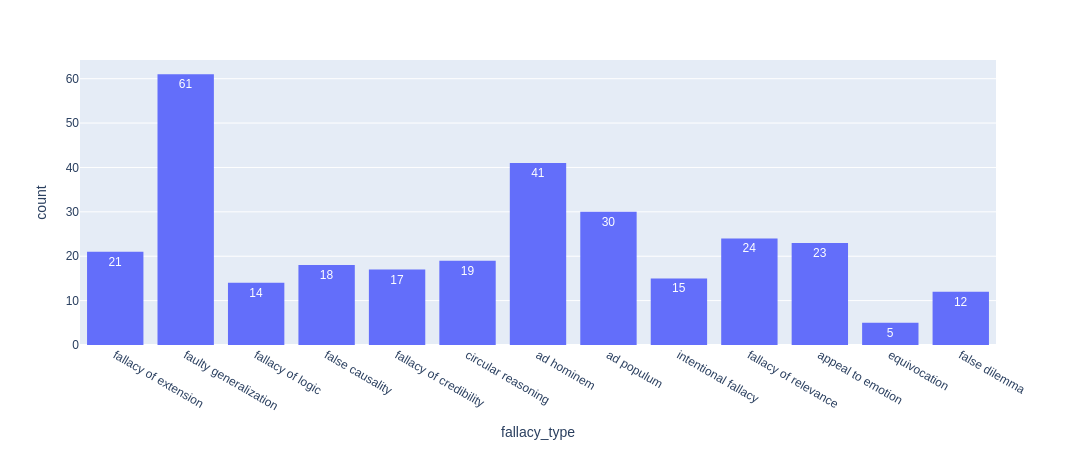
\includegraphics[width=\textwidth]{graphics/fine_grained_distribution.png}
\caption{\textbf{LOGIC Dataset}}
\end{figure}

\begin{figure}[H]
\centering
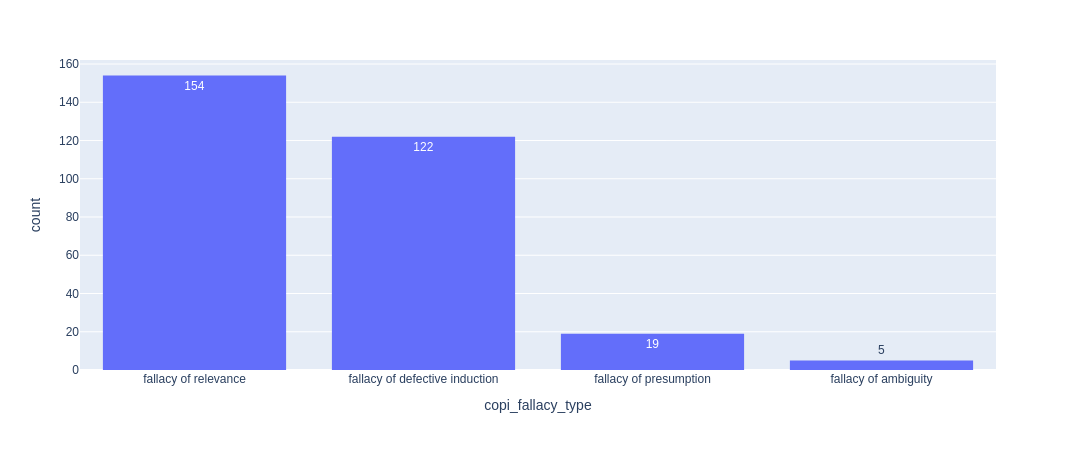
\includegraphics[width=\textwidth]{graphics/copi_distribution.png}
\caption{\textbf{LOGIC Dataset to coarse-grained classes by Copi}}
\end{figure}

\begin{figure}[H]
\centering
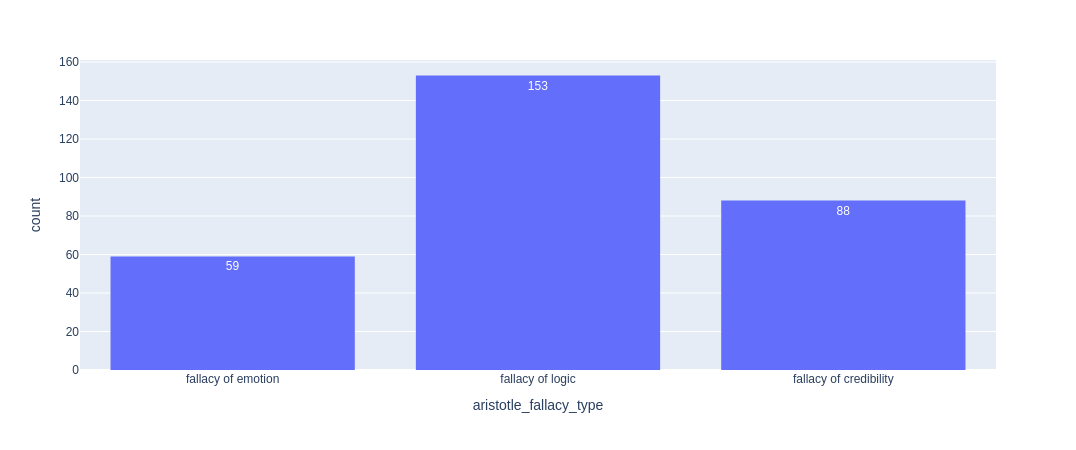
\includegraphics[width=\textwidth]{graphics/aristotle_distribution.png}
\caption{\textbf{LOGIC Dataset to coarse-grained classes by Aristotle}}
\end{figure}

\section{Zero-shot}


\subsection{ Fine Grained Logic Classes}
\begin{table}[H]
\centering
\resizebox{\textwidth}{!}{%
\begin{tabular}{lrrllll}
\toprule
model & def & prompt & accuracy & f1 score & failed & unknown labels \\
\midrule
falcon-mamba-7b-instruct & False & 1 & 21.000 & 0.081 & 2.333 & 7.667 \\
falcon-mamba-7b-instruct & True & 1 & 20.333 & 0.086 & 2.667 & 11.667 \\
Meta-Llama-3.1-8B-Instruct & False & 1 & 40.333 & 0.211 & 0.000 & 2.333 \\
Meta-Llama-3.1-8B-Instruct & True & 1 & 38.333 & 0.208 & 0.000 & 1.667 \\
Mistral-7B-Instruct-v0.3 & False & 1 & 39.333 & 0.153 & 0.000 & 6.333 \\
Mistral-7B-Instruct-v0.3 & True & 1 & 34.667 & 0.210 & 0.000 & 7.333 \\
falcon-mamba-7b-instruct & False & 2 & 24.667 & 0.095 & 6.333 & 9.000 \\
falcon-mamba-7b-instruct & True & 2 & 22.667 & 0.082 & 6.000 & 13.000 \\
Meta-Llama-3.1-8B-Instruct & False & 2 & 40.000 & 0.216 & 0.000 & 2.333 \\
Meta-Llama-3.1-8B-Instruct & True & 2 & \textbf{41.667} & \textbf{0.237} & 0.000 & 1.333 \\
Mistral-7B-Instruct-v0.3 & False & 2 & 39.333 & 0.158 & 0.000 & 4.667 \\
Mistral-7B-Instruct-v0.3 & True & 2 & 33.000 & 0.189 & 0.000 & 8.333 \\
\bottomrule
\end{tabular}}
\caption{Fine-grained Classes Results}
\end{table}

\begin{figure}[H]
\centering
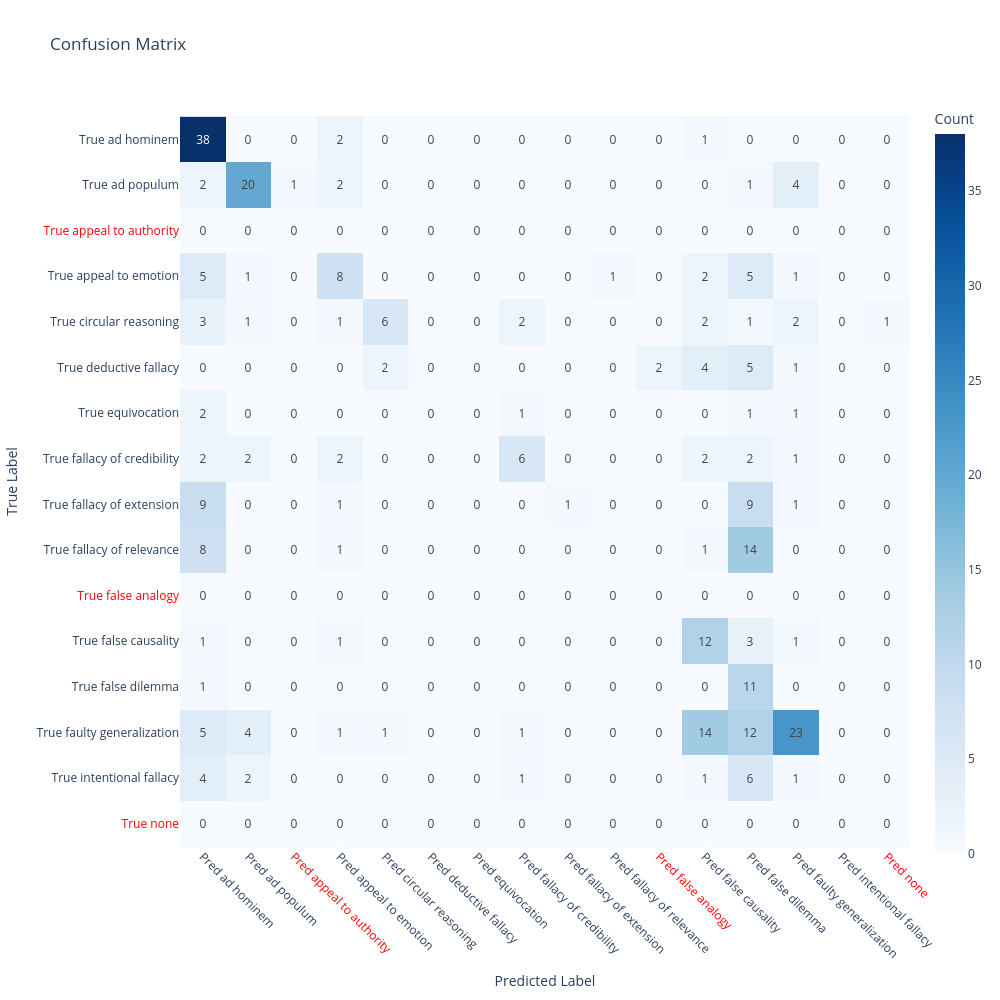
\includegraphics[width=\textwidth]{graphics/conf_matrix_meta-llama-Meta-Llama-3.1-8B-Instruct_prompt2_no_cot_FINE_GRAINED_results_with_definitions_42_no_sampling.png}
\caption{\textbf{Best performing model's results Confusion Matrix}}
\end{figure}


\subsection{ Coarse Grained Copi Classes}
\begin{table}[H]
\centering
\resizebox{\textwidth}{!}{%
\begin{tabular}{lrrllll}
\toprule
model & def & prompt & accuracy & f1 score & failed & unknown \\
\midrule
falcon-mamba-7b-instruct & False & 1 & 43.667 & 0.080 & 2.000 & 2.667 \\
falcon-mamba-7b-instruct & True & 1 & 51.000 & 0.134 & 5.000 & 1.333 \\
Meta-Llama-3.1-8B-Instruct & False & 1 & 55.333 & 0.371 & 0.000 & 0.000 \\
Meta-Llama-3.1-8B-Instruct & True & 1 & \textbf{61.000} & \textbf{0.408} & 0.000 & 0.000 \\
Mistral-7B-Instruct-v0.3 & False & 1 & 44.333 & 0.102 & 0.000 & 4.667 \\
Mistral-7B-Instruct-v0.3 & True & 1 & 50.333 & 0.083 & 0.000 & 2.667 \\
falcon-mamba-7b-instruct & False & 2 & 30.333 & 0.036 & 0.333 & 9.333 \\
falcon-mamba-7b-instruct & True & 2 & 38.667 & 0.056 & 1.000 & 9.000 \\
Meta-Llama-3.1-8B-Instruct & False & 2 & 59.000 & 0.327 & 0.333 & 0.000 \\
Meta-Llama-3.1-8B-Instruct & True & 2 & 54.333 & 0.312 & 0.333 & 0.000 \\
Mistral-7B-Instruct-v0.3 & False & 2 & 33.333 & 0.060 & 0.000 & 11.667 \\
Mistral-7B-Instruct-v0.3 & True & 2 & 47.667 & 0.069 & 0.000 & 12.333 \\
\bottomrule
\end{tabular}}
\caption{Coarse-grained Copi Classes Results}
\end{table}

\begin{figure}[H]
\centering
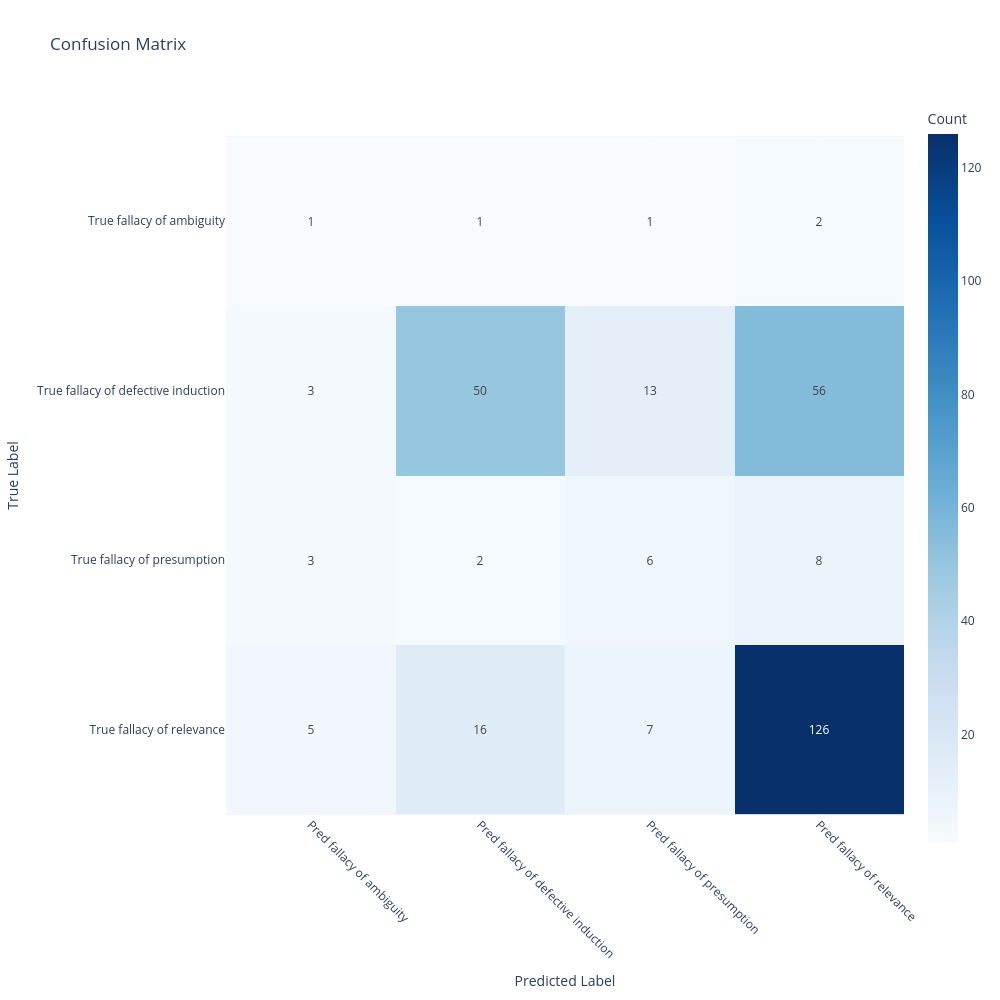
\includegraphics[width=\textwidth]{graphics/conf_matrix_meta-llama-Meta-Llama-3.1-8B-Instruct_prompt1_no_cot_COPI_results_with_definitions_42_no_sampling.png}
\caption{\textbf{Best performing model's results Confusion Matrix}}
\end{figure}

\begin{table}[H]
\centering
\resizebox{\textwidth}{!}{%
\begin{tabular}{lrrllll}
\toprule
model & def & prompt & accuracy & f1 score & failed & unknown \\
\midrule
falcon-mamba-7b-instruct & False & 1 & 54.000 & 0.276 & 10.000 & 0.000 \\
falcon-mamba-7b-instruct & True & 1 & 50.000 & 0.260 & 14.333 & 0.000 \\
Meta-Llama-3.1-8B-Instruct & False & 1 & 67.000 & 0.389 & 2.333 & 0.000 \\
Meta-Llama-3.1-8B-Instruct & True & 1 & 64.000 & 0.380 & 1.667 & 0.000 \\
Mistral-7B-Instruct-v0.3 & False & 1 & 61.000 & 0.332 & 6.333 & 0.000 \\
Mistral-7B-Instruct-v0.3 & True & 1 & 62.333 & 0.359 & 7.333 & 0.000 \\
falcon-mamba-7b-instruct & False & 2 & 52.333 & 0.280 & 15.333 & 0.000 \\
falcon-mamba-7b-instruct & True & 2 & 48.667 & 0.272 & 19.000 & 0.000 \\
Meta-Llama-3.1-8B-Instruct & False & 2 & 64.667 & 0.396 & 2.333 & 0.000 \\
Meta-Llama-3.1-8B-Instruct & True & 2 & \textbf{67.000} & \textbf{0.411} & 1.333 & 0.000 \\
Mistral-7B-Instruct-v0.3 & False & 2 & 64.000 & 0.397 & 4.667 & 0.000 \\
Mistral-7B-Instruct-v0.3 & True & 2 & 60.000 & 0.354 & 8.333 & 0.000 \\
\bottomrule
\end{tabular}}
\caption{Results when mapping fine-grained results to Copi's coarse-grained classes}
\end{table}

\subsection{ Coarse Grained Aritotle Classes}
\begin{table}[H]
\centering
\resizebox{\textwidth}{!}{%
\begin{tabular}{lrrllll}
\toprule
model & def & prompt & accuracy & f1 score & failed & unknown \\
\midrule
falcon-mamba-7b-instruct & False & 1 & 36.333 & 0.127 & 1.333 & 1.667 \\
falcon-mamba-7b-instruct & True & 1 & 34.333 & 0.072 & 1.667 & 5.333 \\
Meta-Llama-3.1-8B-Instruct & False & 1 & \textbf{51.667} & \textbf{0.465} & 0.000 & 0.000 \\
Meta-Llama-3.1-8B-Instruct & True & 1 & 55.667 & 0.303 & 0.000 & 0.667 \\
Mistral-7B-Instruct-v0.3 & False & 1 & 52.333 & 0.116 & 0.000 & 8.000 \\
Mistral-7B-Instruct-v0.3 & True & 1 & 50.667 & 0.116 & 0.000 & 8.333 \\
falcon-mamba-7b-instruct & False & 2 & 41.333 & 0.136 & 0.333 & 2.333 \\
falcon-mamba-7b-instruct & True & 2 & 41.333 & 0.104 & 0.000 & 4.333 \\
Meta-Llama-3.1-8B-Instruct & False & 2 & 41.000 & 0.272 & 0.333 & 0.000 \\
Meta-Llama-3.1-8B-Instruct & True & 2 & 54.333 & 0.292 & 0.333 & 0.333 \\
Mistral-7B-Instruct-v0.3 & False & 2 & 56.333 & 0.094 & 0.000 & 10.000 \\
Mistral-7B-Instruct-v0.3 & True & 2 & 59.667 & 0.285 & 0.000 & 1.667 \\
\bottomrule
\end{tabular}}
\caption{Coarse-grained Aritotle Classes Results}
\end{table}


\begin{figure}[H]
\centering
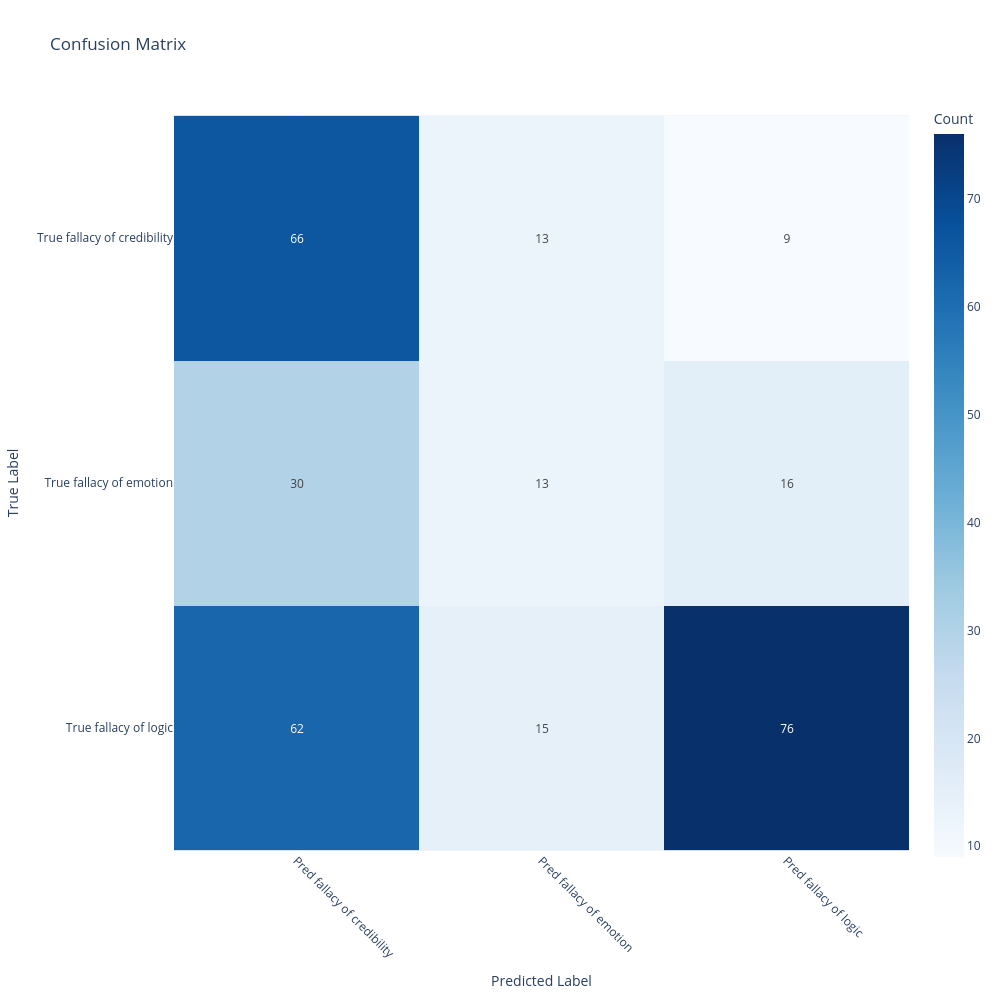
\includegraphics[width=\textwidth]{graphics/conf_matrix_meta-llama-Meta-Llama-3.1-8B-Instruct_prompt1_no_cot_ARISTOTLE_results_no_definitions_42_no_sampling.png}
\caption{\textbf{Best performing model's results Confusion Matrix}}
\end{figure}

\begin{table}[H]
\centering
\resizebox{\textwidth}{!}{%
\begin{tabular}{lrrllll}
\toprule
model & def & prompt & accuracy & f1 score & failed & unknown \\
\midrule
falcon-mamba-7b-instruct & False & 1 & 41.333 & 0.328 & 10.000 & 0.000 \\
falcon-mamba-7b-instruct & True & 1 & 39.000 & 0.303 & 14.333 & 0.000 \\
Meta-Llama-3.1-8B-Instruct & False & 1 & 60.333 & 0.422 & 2.333 & 0.000 \\
Meta-Llama-3.1-8B-Instruct & True & 1 & 60.333 & 0.435 & 1.667 & 0.000 \\
Mistral-7B-Instruct-v0.3 & False & 1 & 57.667 & 0.456 & 6.333 & 0.000 \\
Mistral-7B-Instruct-v0.3 & True & 1 & 53.667 & 0.422 & 7.333 & 0.000 \\
falcon-mamba-7b-instruct & False & 2 & 41.667 & 0.352 & 15.333 & 0.000 \\
falcon-mamba-7b-instruct & True & 2 & 40.000 & 0.329 & 19.000 & 0.000 \\
Meta-Llama-3.1-8B-Instruct & False & 2 & \textbf{63.333} & 0.446 & 2.333 & 0.000 \\
Meta-Llama-3.1-8B-Instruct & True & 2 & 62.333 & \textbf{0.465} & 1.333 & 0.000 \\
Mistral-7B-Instruct-v0.3 & False & 2 & 59.333 & 0.402 & 4.667 & 0.000 \\
Mistral-7B-Instruct-v0.3 & True & 2 & 52.333 & 0.360 & 8.333 & 0.000 \\
\bottomrule
\end{tabular}}
\caption{Results when mapping fine-grained results to Aritotle's coarse-grained classes}
\end{table}









\section{Basic CoT}

\subsection{ Fine Grained Logic Classes}
\begin{table}[H]
\centering
\caption{Fine-grained Classes Results}
\resizebox{\textwidth}{!}{%
\begin{tabular}{lrrllll}
\toprule
model & def & prompt & accuracy & f1 score & failed & unknown \\
\midrule
falcon-mamba-7b-instruct & False & 1 & 17.667 & 0.062 & 5.000 & 9.000 \\
falcon-mamba-7b-instruct & True & 1 & 18.333 & 0.081 & 0.333 & 5.333 \\
Meta-Llama-3.1-8B-Instruct & False & 1 & 39.333 & 0.213 & 0.000 & 3.000 \\
Meta-Llama-3.1-8B-Instruct & True & 1 & 36.667 & 0.251 & 0.000 & 0.333 \\
Mistral-7B-Instruct-v0.3 & False & 1 & 39.667 & 0.161 & 0.000 & 5.333 \\
Mistral-7B-Instruct-v0.3 & True & 1 & 34.333 & 0.198 & 0.000 & 7.333 \\
falcon-mamba-7b-instruct & False & 2 & 22.667 & 0.087 & 2.333 & 10.000 \\
falcon-mamba-7b-instruct & True & 2 & 23.000 & 0.081 & 3.000 & 15.000 \\
Meta-Llama-3.1-8B-Instruct & False & 2 & 41.000 & 0.230 & 0.000 & 3.000 \\
Meta-Llama-3.1-8B-Instruct & True & 2 & \textbf{42.000} & \textbf{0.266} & 0.000 & 0.667 \\
Mistral-7B-Instruct-v0.3 & False & 2 & 37.667 & 0.171 & 0.000 & 5.000 \\
Mistral-7B-Instruct-v0.3 & True & 2 & 32.333 & 0.162 & 0.000 & 7.333 \\
\bottomrule
\end{tabular}}
\caption{Fine-grained Classes Results}
\end{table}



\subsection{ Coarse Grained Copi Classes}
\begin{table}[H]
\centering
\resizebox{\textwidth}{!}{%
\begin{tabular}{lrrllll}
\toprule
model & def & prompt & accuracy & f1 score & failed & unknown \\
\midrule
falcon-mamba-7b-instruct & False & 1 & 49.333 & 0.102 & 2.667 & 3.000 \\
falcon-mamba-7b-instruct & True & 1 & 53.333 & 0.132 & 1.000 & 0.667 \\
Meta-Llama-3.1-8B-Instruct & False & 1 & 59.667 & \textbf{0.405} & 0.000 & 0.000 \\
Meta-Llama-3.1-8B-Instruct & True & 1 & \textbf{61.000} & 0.403 & 0.000 & 0.000 \\
Mistral-7B-Instruct-v0.3 & False & 1 & 38.667 & 0.089 & 0.000 & 3.667 \\
Mistral-7B-Instruct-v0.3 & True & 1 & 50.667 & 0.102 & 0.000 & 1.667 \\
falcon-mamba-7b-instruct & False & 2 & 34.667 & 0.071 & 2.667 & 5.667 \\
falcon-mamba-7b-instruct & True & 2 & 38.333 & 0.070 & 0.000 & 12.333 \\
Meta-Llama-3.1-8B-Instruct & False & 2 & 58.000 & 0.388 & 0.000 & 0.000 \\
Meta-Llama-3.1-8B-Instruct & True & 2 & 51.333 & 0.284 & 0.333 & 0.000 \\
Mistral-7B-Instruct-v0.3 & False & 2 & 30.667 & 0.051 & 0.000 & 12.000 \\
Mistral-7B-Instruct-v0.3 & True & 2 & 43.667 & 0.064 & 0.000 & 13.333 \\
\bottomrule
\end{tabular}}
\caption{Coarse-grained Copi Classes Results}
\end{table}



\subsection{ Coarse Grained Aritotle Classes}
\begin{table}[H]
\centering
\resizebox{\textwidth}{!}{%
\begin{tabular}{lrrllll}
\toprule
model & def & prompt & accuracy & f1 score & failed & unknown \\
\midrule
falcon-mamba-7b-instruct & False & 1 & 27.333 & 0.078 & 3.333 & 3.333 \\
falcon-mamba-7b-instruct & True & 1 & 29.667 & 0.079 & 1.000 & 2.333 \\
Meta-Llama-3.1-8B-Instruct & False & 1 & 52.667 & \textbf{0.437} & 0.000 & 0.000 \\
Meta-Llama-3.1-8B-Instruct & True & 1 & \textbf{58.000} & 0.379 & 0.333 & 0.000 \\
Mistral-7B-Instruct-v0.3 & False & 1 & 55.667 & 0.158 & 0.000 & 4.333 \\
Mistral-7B-Instruct-v0.3 & True & 1 & 55.000 & 0.175 & 0.000 & 4.667 \\
falcon-mamba-7b-instruct & False & 2 & 38.000 & 0.137 & 1.000 & 1.333 \\
falcon-mamba-7b-instruct & True & 2 & 39.333 & 0.085 & 0.667 & 3.333 \\
Meta-Llama-3.1-8B-Instruct & False & 2 & 39.000 & 0.253 & 0.333 & 0.000 \\
Meta-Llama-3.1-8B-Instruct & True & 2 & 53.667 & 0.377 & 0.333 & 0.000 \\
Mistral-7B-Instruct-v0.3 & False & 2 & 54.000 & 0.091 & 0.000 & 10.333 \\
Mistral-7B-Instruct-v0.3 & True & 2 & 59.000 & 0.190 & 0.000 & 3.000 \\
\bottomrule
\end{tabular}}
\caption{Coarse-grained Aritotle Classes Results}
\end{table}


\begin{table} [H]
\centering
\resizebox{\textwidth}{!}{%
\begin{tabular}{lrrllll}
\toprule
model & def & prompt & acc & f1 & failed & unknown \\
\midrule
falcon-mamba-7b-instruct & False & 1 & 46.333 & 0.199 & 14.000 & 0.000 \\
falcon-mamba-7b-instruct & True & 1 & 49.333 & 0.221 & 5.667 & 0.000 \\
Meta-Llama-3.1-8B-Instruct & False & 1 & 65.667 & 0.414 & 3.000 & 0.000 \\
Meta-Llama-3.1-8B-Instruct & True & 1 & 60.000 & 0.367 & 0.333 & 0.000 \\
Mistral-7B-Instruct-v0.3 & False & 1 & 63.333 & 0.358 & 5.333 & 0.000 \\
Mistral-7B-Instruct-v0.3 & True & 1 & 63.000 & 0.362 & 7.333 & 0.000 \\
falcon-mamba-7b-instruct & False & 2 & 51.000 & 0.266 & 12.333 & 0.000 \\
falcon-mamba-7b-instruct & True & 2 & 48.333 & 0.286 & 18.000 & 0.000 \\
Meta-Llama-3.1-8B-Instruct & False & 2 & \textbf{67.667} & \textbf{0.428} & 3.000 & 0.000 \\
Meta-Llama-3.1-8B-Instruct & True & 2 & 66.667 & 0.398 & 0.667 & 0.000 \\
Mistral-7B-Instruct-v0.3 & False & 2 & 64.333 & 0.430 & 5.000 & 0.000 \\
Mistral-7B-Instruct-v0.3 & True & 2 & 62.333 & 0.341 & 7.333 & 0.000 \\
\bottomrule
\end{tabular}}
\caption{COPI Coarse-Grained to Fine-Grained Basic CoT}
\end{table}

\begin{table}[H]
\centering
\resizebox{\textwidth}{!}{%
\begin{tabular}{lrrllll}
\toprule
model & def & prompt & acc & f1 & failed & unknown \\
\midrule
falcon-mamba-7b-instruct & False & 1 & 37.667 & 0.316 & 14.000 & 0.000 \\
falcon-mamba-7b-instruct & True & 1 & 45.667 & 0.342 & 5.667 & 0.000 \\
Meta-Llama-3.1-8B-Instruct & False & 1 & 59.667 & 0.398 & 3.000 & 0.000 \\
Meta-Llama-3.1-8B-Instruct & True & 1 & 60.667 & 0.427 & 0.333 & 0.000 \\
Mistral-7B-Instruct-v0.3 & False & 1 & 58.333 & 0.459 & 5.333 & 0.000 \\
Mistral-7B-Instruct-v0.3 & True & 1 & 53.333 & 0.420 & 7.333 & 0.000 \\
falcon-mamba-7b-instruct & False & 2 & 36.667 & 0.312 & 12.333 & 0.000 \\
falcon-mamba-7b-instruct & True & 2 & 38.667 & 0.317 & 18.000 & 0.000 \\
Meta-Llama-3.1-8B-Instruct & False & 2 & \textbf{63.333} & \textbf{0.465} & 3.000 & 0.000 \\
Meta-Llama-3.1-8B-Instruct & True & 2 & 61.667 & 0.425 & 0.667 & 0.000 \\
Mistral-7B-Instruct-v0.3 & False & 2 & 56.667 & 0.372 & 5.000 & 0.000 \\
Mistral-7B-Instruct-v0.3 & True & 2 & 50.333 & 0.331 & 7.333 & 0.000 \\
\bottomrule
\end{tabular}}
\caption{ARISTOTLE Coarse-Grained to Fine-Grained Basic CoT}
\end{table}





\section{Multi-Round CoT (From Coarse-Grained to Fine-Grained)}




\begin{table} [H]
\centering
\resizebox{\textwidth}{!}{%
\begin{tabular}{lrrllllll}
\toprule
model & def & prompt & r1\_accuracy & r1\_f1 & acc & f1 & failed & unknown \\
\midrule
falcon-mamba-7b-instruct & False & 1 & 35.333 & 0.053 & 5.000 & 0.032 & 0.333 & 60.000 \\
falcon-mamba-7b-instruct & True & 1 & 47.000 & 0.082 & 7.000 & 0.025 & 0.333 & 53.000 \\
Meta-Llama-3.1-8B-Instruct & False & 1 & 55.000 & 0.376 & 32.667 & 0.213 & 0.000 & 1.333 \\
Meta-Llama-3.1-8B-Instruct & True & 1 & 57.333 & 0.379 & 31.667 & 0.212 & 0.000 & 1.333 \\
Mistral-7B-Instruct-v0.3 & False & 1 & 39.333 & 0.051 & 30.333 & 0.179 & 0.000 & 1.333 \\
Mistral-7B-Instruct-v0.3 & True & 1 & 49.667 & 0.057 & 28.667 & 0.176 & 0.000 & 1.333 \\
falcon-mamba-7b-instruct & False & 2 & 25.333 & 0.031 & 8.333 & 0.045 & 0.000 & 50.333 \\
falcon-mamba-7b-instruct & True & 2 & 38.333 & 0.047 & 11.333 & 0.051 & 0.000 & 29.333 \\
Meta-Llama-3.1-8B-Instruct & False & 2 & 56.333 & 0.390 & 32.000 & 0.231 & 0.000 & 0.333 \\
Meta-Llama-3.1-8B-Instruct & True & 2 & 50.000 & 0.359 & \textbf{32.667} & \textbf{0.247} & 0.000 & 0.667 \\
Mistral-7B-Instruct-v0.3 & False & 2 & 32.667 & 0.042 & 31.000 & 0.157 & 0.000 & 1.667 \\
Mistral-7B-Instruct-v0.3 & True & 2 & 44.667 & 0.053 & 34.333 & 0.160 & 0.000 & 4.333 \\
\bottomrule
\end{tabular}
}
\caption{COPI Coarse-Grained to Fine-Grained Multi-round CoT}
\end{table}

\begin{table}[H]
\centering
\resizebox{\textwidth}{!}{%
\begin{tabular}{lrrllllll}
\toprule
model & def & prompt & r1\_accuracy & r1\_f1 & acc & f1 & failed & unknown \\
\midrule
falcon-mamba-7b-instruct & False & 1 & 42.000 & 0.139 & 7.333 & 0.035 & 0.333 & 31.000 \\
falcon-mamba-7b-instruct & True & 1 & 39.000 & 0.055 & 10.333 & 0.054 & 0.333 & 20.667 \\
Meta-Llama-3.1-8B-Instruct & False & 1 & 56.000 & 0.470 & 32.333 & 0.215 & 0.000 & 1.000 \\
Meta-Llama-3.1-8B-Instruct & True & 1 & 55.667 & 0.500 & 32.000 & 0.233 & 0.000 & 3.333 \\
Mistral-7B-Instruct-v0.3 & False & 1 & 43.667 & 0.032 & 35.333 & 0.128 & 0.000 & 5.000 \\
Mistral-7B-Instruct-v0.3 & True & 1 & 50.000 & 0.048 & 26.667 & 0.134 & 0.000 & 7.000 \\
falcon-mamba-7b-instruct & False & 2 & 43.000 & 0.099 & 7.667 & 0.043 & 0.000 & 39.333 \\
falcon-mamba-7b-instruct & True & 2 & 38.667 & 0.076 & 11.667 & 0.069 & 0.000 & 18.000 \\
Meta-Llama-3.1-8B-Instruct & False & 2 & 44.667 & 0.411 & 30.333 & 0.196 & 0.000 & 1.000 \\
Meta-Llama-3.1-8B-Instruct & True & 2 & 56.333 & 0.382 & 35.333 & \textbf{0.250} & 0.000 & 4.333 \\
Mistral-7B-Instruct-v0.3 & False & 2 & 43.333 & 0.040 & \textbf{35.667} & 0.188 & 0.000 & 3.000 \\
Mistral-7B-Instruct-v0.3 & True & 2 & 52.000 & 0.096 & 31.333 & 0.175 & 0.000 & 11.333 \\
\bottomrule
\end{tabular}
}
\caption{ARISTOTLE Coarse-Grained to Fine-Grained Multi-round CoT}
\end{table} 
%!TEX root = ../Thesis.tex
\chapter{Conclusion} \label{Conclusion}

\chapter{Future Work}



%\include{chapters/LongTitle}
%\blinddocument

\printbibliography


\appendix 
%\addcontentsline{toc}{section}{Nomenclature}
%%!TEX root = ../Thesis.tex


\chapter{Python Scripts}

Appendix A includes all the developed Python scripts throughout this study. 


%C.1includes the scripts for the simulation and damage assessment of the 3D steel frame,
%while C.2 includes the corresponding scripts for the offshore wind turbine.

\newpage
\begin{lstlisting}[language=Python, caption = Python Script that create plots for all different scenario's, label=lst:plots]
#Python Script that create plots for all different scenario's
#Import all the important packets
import pandas as pd 
import matplotlib.pyplot as plt 
import seaborn as sns
import matplotlib as mpl
import numpy as np
import matplotlib.cm

#Read all the data from the file
df1=pd.read_excel('DataScenarios.xlsx', index_col=0)

df_list=[]
for i in df1['dfid'].unique():
    x='df'+str(i)
    x=df1[df1['dfid'] == i]
    df_list.append(x)
    
sns.set(style="darkgrid")

#add colors
colors = ['#4daf4a','#e41a1d']
mylabels = ["Successful","Unsuccessful"]
       
fig, ax = plt.subplots()
###########################################################################
for df in df_list:

    for percentage in df.Percentage:
        plt.pie([percentage,100.0 - percentage], autopct='%.2f%%', shadow=True, startangle=90, colors = colors, labels = mylabels)
        plt.legend()
        plt.xlabel('Successful Transmissions')
        plt.show() 
    index = range(1,len(df)+1)
    array = []
    for i in index:
        array.append(i) 

    fig, ax = plt.subplots()
    pps = plt.bar(array, df.Percentage, align = 'center', alpha = 0.5, color = 'maroon', width = 0.5)
    plt.xticks(array)
    plt.ylabel('Successful Transmissions')
    plt.title("Successful Rate in Different Experiments")
    for p in pps:
        height = p.get_height()
        ax.text(x=p.get_x() + p.get_width() / 2, y=height+.10, s="{}%".format(height), ha='center',  weight='bold')
    plt.show()
    
\end{lstlisting}
\newpage
\begin{lstlisting}[language=Python, caption = Python Script that search for duplications\, check for successful transmissions and find out the overall and individual node PDRs, label=lst:DER]
#Python Script that search for duplications, check for successful transmissions and find out the overall and individual node DERs.
#Import all the important packets
import re
import subprocess
import pandas as pd
from collections import Counter

class bcolors:
    HEADER = '\033[95m'
    OKBLUE = '\033[94m'
    OKCYAN = '\033[96m'
    OKGREEN = '\033[92m'
    WARNING = '\033[93m'
    FAIL = '\033[91m'
    ENDC = '\033[0m'
    BOLD = '\033[1m'
    UNDERLINE = '\033[4m'

df = pd.DataFrame(columns=['intersections', 'total', 'Percentage'])
NODE_NUM = 5

# for all nodes
for node in range(NODE_NUM): 
    # get output from grep commands and transform into utf8
    data = subprocess.Popen(['grep "LoRaGWRadio Reception ended: successfully for" logn5tractormobgw1-29.elog | grep "transmissionId"'], shell=True, stdout = subprocess.PIPE)
    data1 = subprocess.Popen([f'grep "Transmission started:" logn5tractormobgw1-29.elog | grep "transmitterId = {node}" | grep "id"'], shell=True, stdout = subprocess.PIPE)
    output = data.stdout.read().decode("utf-8")
    output1 = data1.stdout.read().decode("utf-8")

    rids = [] # receiver ids
    intersection = [] # the match between rids and tids
    tids = set() # node duplicates distinct and unordered / transmission ids

    print('{}Searching logfile...{}'
                .format(bcolors.HEADER, bcolors.ENDC))
    # split grep command output on transmissionid and get second part
    for i, item in enumerate(output.split("transmissionId")):
        if i == 0:
            continue
        
        # get 1st and 2nd numbers with regular expressions
        tid = re.search(r'\d+', item).group()
        rid = re.search(r'\d+', item[10:]).group()
        
        # check for successful transmissions by matching the previous in the other grep command 
        for j, item in enumerate(output1.split("id")):
                if j == 0:
                    continue

                ida = re.search(r'\d+', item).group()

                if ida == tid :
                    #print(f'Node {node} send and Found ID: {ida}')
                    intersection.append(ida)


        #print(f'TID: {tid} \t RID: {rid}')
        rids.append(rid)
        tids.add(tid)


    # casting to a set to get unique values    
    intersection_set = set(intersection)
    print(f'Intersection on node {node}: {len(intersection_set)}')
    # Filing the DataFrame with per node PRR 
    df.loc[node] = [len(intersection_set), j, len(intersection_set) / j*100] # j is the total for each node 

# Export the dataframe to an excel 
df.index.name = 'node'
df.to_excel("output_nodes_stats.xlsx")

print(df)
print(f'\nCummulative successfull transmission count: {len(rids)}\nIndividual count: {Counter(rids)}')
print(f'Successfull non-duplicated transmissions: {len(tids)}')    

# Getting the total from mystats ( mystats.txt is created with a custom script embedded in the simulator code)
cmdout = subprocess.Popen(['cat mystats.txt'], shell=True, stdout = subprocess.PIPE)
cmdout_proc = cmdout.stdout.read().decode("utf-8")
total = int(re.search(r'\d+', cmdout_proc).group())

print(f'Total transmissions: {total}')

percentage = len(tids) / total * 100
print('{}{}Successfull transmission percentage: {:.2f}%{}{}'
            .format(bcolors.BOLD, bcolors.OKGREEN, percentage, bcolors.ENDC, bcolors.ENDC))
\end{lstlisting}




\newpage
\begin{lstlisting}[language=Python, caption = Python Script that visualize the results with standard deviation error bars, label=lst:ploteachnode]
#Python Script that visualize the results with standard deviation error bars.
#Import all the important packets
import pandas as pd 
import matplotlib.pyplot as plt 
import seaborn as sns
import matplotlib as mpl
import numpy as np
import matplotlib.cm


 
node_stats = pd.read_excel('tractor_merged.xlsx', index_col=[0])
# for x nodes
x=16
node_list=[]
for i in range(x):
  node_list.append(node_stats.loc[node_stats['node'] == i])

node_percentages=[]
for item in node_list:
  node_percentages.append(item['Percentage'].to_numpy())

node_averages=[]
for item in node_percentages:
  node_averages.append(np.mean(item))

node_stds = []
for item in node_percentages:
  node_stds.append(np.std(item))

nodes=[]
for i in range(x):
  nodes.append(str(i))

x_pos = np.arange(len(nodes))
CTEs = node_averages
error = node_stds

sns.set()
fig, ax = plt.subplots(figsize=(12, 6))
plt.ylim([0, 100])


df = pd.DataFrame(node_averages,columns=['Percentage'])
#print(df)
df.to_excel("final_percentages.xlsx")                    

pps = ax.bar(x_pos, CTEs, yerr=error, align='center', alpha=0.5, ecolor='maroon', capsize=10, width = 0.5)
for p in pps:
    height = p.get_height()
    ax.text(x=p.get_x() + p.get_width() / 2, y=height+ 4, s="{:.2f}%".format(height), ha='center',  weight='bold')

#ax.text(4.5, 100, 'Jain\'s fairness \nindex = 0.8744', size=15, color='purple')    
ax.set_ylabel('Packet Delivery Rate / PDR')
ax.set_xticks(x_pos)
ax.set_xticklabels(nodes)
ax.set_xlabel('Nodes')
ax.set_title('Successful Rate on each node')


# Save the figure and show
plt.tight_layout()
plt.savefig('bar_plot_with_error_bars.png')
plt.show()
 
\end{lstlisting}

\begin{lstlisting}[language=Python, caption = Python Script that calculates Jain's fairness index, label=lst:jindex]
#Python Script that calculates Jain's fairness index.
#Import all the important packets
import pandas as pd 
import matplotlib.pyplot as plt 
import seaborn as sns
import matplotlib as mpl
import numpy as np
import matplotlib.cm

#throughputs = [0.4244, 0.4942, 0.3314, 0.3140, 0.4128]
df1=pd.read_excel('output_nodes_stats_1gw.xlsx', index_col=0)
throughputs=df1['Percentage'].div(100).round(4).tolist()
throughputs

def jains_fairness_index(throughputs):
        
    n = len(throughputs)
    temp = sum([ (x**2) for x in throughputs])
    jains_index = sum(throughputs) ** 2 / (n * temp)
 
    return jains_index


jains_index = jains_fairness_index(throughputs)
print(jains_index)
\end{lstlisting}


All the files with the source code and the python scripts can be found in this \href{https://github.com/memorial4/LoRa_Mobility}{link}.



%\chapter{Lora Range in Simulator}

Appendix b includes all the  figures related to the Lora range of the simulator and framework flora. 


\begin{figure}[H]
    \centering
      \includegraphics[width=0.8\textwidth]{graphics/range/Figure_1.png}
      \caption{Coverage of GW with SF = 7 and TP = 14}
      \label{fig:fig1}
\end{figure}

\begin{figure}[H]
    \centering
      \includegraphics[width=0.8\textwidth]{graphics/range/Figure_2.png}
      \caption{Coverage of GW with SF = 8 and TP = 14}
      \label{fig:fig2}
\end{figure}

\begin{figure}[H]
    \centering
      \includegraphics[width=0.8\textwidth]{graphics/range/Figure_3.png}
      \caption{Coverage of GW with SF = 9 and TP = 14}
      \label{fig:fig3}
\end{figure}

\begin{figure}[H]
    \centering
      \includegraphics[width=0.8\textwidth]{graphics/range/Figure_4.png}
      \caption{Coverage of GW with SF = 10 and TP = 14}
      \label{fig:fig4}
\end{figure}

\begin{figure}[H]
    \centering
      \includegraphics[width=0.8\textwidth]{graphics/range/Figure_5.png}
      \caption{Coverage of GW with SF = 11 and TP = 14}
      \label{fig:fig5}
\end{figure}

\begin{figure}[H]
    \centering
      \includegraphics[width=0.8\textwidth]{graphics/range/Figure_6.png}
      \caption{Coverage of GW with SF = 12 and TP = 14}
      \label{fig:fig6}
\end{figure}

\begin{figure}[H]
    \centering
      \includegraphics[width=0.8\textwidth]{graphics/range/Figure_7.png}
      \caption{Coverage of GW with SF = 12 and TP = 17}
      \label{fig:fig7}
\end{figure}

\begin{figure}[H]
    \centering
      \includegraphics[width=0.8\textwidth]{graphics/range/Figure_8.png}
      \caption{Coverage of GW with SF = 11 and TP = 17}
      \label{fig:fig8}
\end{figure}

\begin{figure}[H]
    \centering
      \includegraphics[width=0.8\textwidth]{graphics/range/Figure_9.png}
      \caption{Coverage of GW with SF = 10 and TP = 17}
      \label{fig:fig9}
\end{figure}

\begin{figure}[H]
    \centering
      \includegraphics[width=0.8\textwidth]{graphics/range/Figure_10.png}
      \caption{Coverage of GW with SF = 9 and TP = 17}
      \label{fig:fig10}
\end{figure}

\begin{figure}[H]
    \centering
      \includegraphics[width=0.8\textwidth]{graphics/range/Figure_11.png}
      \caption{Coverage of GW with SF = 8 and TP = 17}
      \label{fig:fig11}
\end{figure}

\begin{figure}[H]
    \centering
      \includegraphics[width=0.8\textwidth]{graphics/range/Figure_12.png}
      \caption{Coverage of GW with SF = 7 and TP = 17}
      \label{fig:fig12}
\end{figure}

\begin{figure}[H]
    \centering
      \includegraphics[width=\textwidth]{graphics/range/Figure_13.png}
      \caption{Coverage of GW with all different SFs and TPs}
      \label{fig:fig13}
\end{figure}


%\backmatter  
%\bibliographystyle{ieeetr}


\end{document}
